\documentclass[a4paper,landscape,8pt]{extarticle}

\usepackage[a4paper,margin=0.7cm]{geometry}

\usepackage{fancyhdr}
\pagestyle{fancy}
\fancyfoot[R]{\vspace{-35pt}\Huge\thepage}

\usepackage{multicol}
\setlength\columnsep{20pt}
\setlength{\columnseprule}{0.1pt} 

\setlength\parindent{0pt}

\usepackage[ngerman]{babel} % Silbentrennung
\usepackage[utf8]{inputenc} % Umlaute
\usepackage{microtype}

\usepackage{hyperref}

\usepackage{float}
\usepackage{graphicx}

\usepackage{comment}
\usepackage{amsmath}
\usepackage{amssymb}

\usepackage{cancel}

\usepackage{color}
\usepackage{xcolor}

\usepackage{color}

\usepackage{booktabs}

\newenvironment{rcases}
  {\left.\begin{aligned}}
  {\end{aligned}\right\rbrace}
  
\usepackage{enumitem}
\setlist{noitemsep,topsep=3pt,parsep=3pt,partopsep=3pt,leftmargin=18pt}
\renewcommand\labelitemi{{\boldmath$\cdot$}}
\newcommand{\listarrow}{
\smash{\scalebox{1.5}[1.75]{\rotatebox[origin=c]{180}{$\Lsh$}}}
}

\usepackage{xifthen}
\newcommand{\emptyarg}[1][]{\ifthenelse{\isempty{#1}}{}{\ #1}}

% % % % %
% Structural
% % % % %

\newcommand{\Def}[1][]{\colorbox{defcolor}{\color{titlecolor}{\textbf{D\emptyarg[#1]}}}\kern+0.3ex}

\newcommand{\Satz}[1][]{\colorbox{satzcolor}{\color{titlecolor}{\textbf{S\emptyarg[#1]}}}\kern+0.3ex}

\newcommand{\Lemma}[1][]{\colorbox{lemcolor}{\color{titlecolor}{\textbf{L\emptyarg[#1]}}}\kern+0.3ex}

\newcommand{\Korollar}[1][]{\colorbox{lemcolor}{\color{titlecolor}{\textbf{K\emptyarg[#1]}}}\kern+0.3ex}

\newcommand{\Trick}[1][]{\colorbox{trkcolor}{\color{titlecolor}{\textbf{Trick:\emptyarg[#1]}}}\kern+0.3ex}

\newcommand{\Vorgehen}[1][]{\colorbox{trkcolor}{\color{titlecolor}{\textbf{Vorgehen:\emptyarg[#1]}}}\kern+0.3ex}

\newcommand{\Bsp}[1][]{\colorbox{bspcolor}{\color{titlecolor}{\textbf{B\emptyarg[#1]}}}\kern+0.3ex}

% % % % %
% In Text
% % % % %

\newcommand{\Bem}{\textbf{Bem: }}
\newcommand{\Beweis}{\textbf{Beweis: }}
\newcommand{\Achtung}{\textbf{Achtung: }}
\newcommand{\Wichtig}{\textbf{Wichtig: }}

% % % % %
% Colors
% % % % %

\definecolor{defcolor}{rgb}{0.5, 1, 0.5}
\definecolor{satzcolor}{rgb}{0.5, 0.95, 1}
\definecolor{lemcolor}{rgb}{1, 0.75, 0.75}
%\definecolor{trkcolor}{rgb}{1, 0.7, 0}
\definecolor{trkcolor}{rgb}{0.7, 0.95, 1}
\definecolor{bspcolor}{rgb}{1, 0.95, 0.43}
\definecolor{titlecolor}{rgb}{0,0,0}

% % % % %
% Math
% % % % %

\DeclareMathOperator{\arcsinh}{arcsinh}
\DeclareMathOperator{\arccosh}{arccosh}
\DeclareMathOperator{\arctanh}{arctanh}
\DeclareMathOperator{\arc}{arc}

\renewcommand\div{\operatorname{div}}
\DeclareMathOperator{\rot}{rot}
\newcommand{\laplace}{\Delta}

\DeclareMathOperator{\cis}{cis}

\DeclareMathOperator{\grad}{grad}
\DeclareMathOperator{\Hess}{Hess}

\newcommand{\N}{\mathbb{N}}
\newcommand{\Z}{\mathbb{Z}}
\newcommand{\Q}{\mathbb{Q}}
\newcommand{\R}{\mathbb{R}}
\newcommand{\C}{\mathbb{C}}

\renewcommand\Re{\operatorname{Re}}
\renewcommand\Im{\operatorname{Im}}

\newcommand{\abs}[1]{\left\lvert #1 \right\rvert}
\newcommand{\norm}[1]{\left\lVert #1 \right\rVert}
\newcommand{\scprod}[1]{\left\langle #1 \right\rangle}
\newcommand{\ceil}[1]{\left\lceil #1 \right\rceil}
\newcommand{\floor}[1]{\left\lfloor #1 \right\rfloor}

\newcommand{\diag}{\operatorname{diag}}

\newcommand{\hl}[1]{\colorbox{black!7}{$#1$}}

\newcommand{\notimplies}{\;\not\!\!\!\implies}

% % % % %
% Layout
% % % % %

\newcommand{\setsep}{\ \vert \ }

\newcommand{\todo}{\textcolor{red}{TODO }}

\newcommand{\sep}{\vspace{5pt}\noindent\hrule\vspace{5pt}}


\newcommand{\veryshortarrow}[1][3pt]{\mathrel{%
   \hbox{\rule[\dimexpr\fontdimen22\textfont2-.2pt\relax]{#1}{.4pt}}%
   \mkern-4mu\hbox{\usefont{U}{lasy}{m}{n}\symbol{41}}}}


% TODO remove command
\renewcommand*{\newpage}{ \ }

%\renewcommand*{\part}{\ }


% package to define custom environments
\usepackage{environ}

% boolean variable to show contents
\newif\ifshowwarmup
%\showwarmuptrue % set it to true
\showwarmupfalse % set it to false

% definition of custom environment
\NewEnviron{warmup}{\ifshowwarmup \BODY \fi}

% shorthand for custom environment
%\def\WU#1\UW{\begin{warmup}#1\end{warmup}}

% Ultra shortening of Document
%
% http://www.terminally-incoherent.com/blog/
%2007/09/19/latex-squeezing-the-vertical-white-space/
%\setlength{\parskip}{0pt}
%\setlength{\parsep}{0pt}
%\setlength{\headsep}{0pt}
\setlength{\topskip}{0pt}
%\setlength{\topmargin}{0pt}
%\setlength{\topsep}{0pt}
%\setlength{\partopsep}{0pt}
%\linespread{0.7}
\usepackage[compact]{titlesec}
\titlespacing{\section}{0pt}{*0}{*0}
\titlespacing{\subsection}{0pt}{*0}{*0}
\titlespacing{\subsubsection}{0pt}{*0}{*0}
%\usepackage{savetrees} %(alternative)

\pagenumbering{gobble}

% Use custom numbering
%\setcounter{secnumdepth}{0}

\usepackage{centernot}

\begin{document}

\setlength{\belowdisplayskip}{4pt} \setlength{\belowdisplayshortskip}{4pt}
\setlength{\abovedisplayskip}{4pt} \setlength{\abovedisplayshortskip}{4pt}

% allow page break in align* environment
\allowdisplaybreaks

\begin{multicols*}{4} % change to 3 if you want only 3 columns
\raggedcolumns

\graphicspath{ {./img/} }

\sep
\section{Grundlagen}
\Satz[1.1] Es gibt keine Gleichung der Form  \[x^n + a_{n-1}x^{n-1}+...+a_0 = 0\]
mit \(a_i \in \Q \), so dass \(x = \pi\) eine Lösung ist \newline
\Satz[1.2] \(R\) ist ein kommutativer, angeordneter Körper, der ordnungsvollständig ist \newline
\Def[Axiome der Addition]
\begin{enumerate}
    \item [A1] Assoziativität \(x+(y+z) = (x+y)+z\)
    \item [A2] Neutrales Element \(x + 0 = x \quad \forall x \in \R\)
    \item [A3] Inverses Element \(\forall x \in \R \  \exists y \in \R: x+y=0\)
    \item [A4] Kommutativität \(x + z = z + x \quad \forall x,z \in \R \)
\end{enumerate}
\Def[Axiome der Multiplikation]
\begin{enumerate}
    \item[M1] Assoziativität \(x \cdot (y \cdot z) = (x \cdot y) \cdot z \quad \forall x,y,z \in R\)
    \item[M2] Neutrales Element \(x \cdot 1 = x \quad \forall x \in \R \)
    \item[M3] Inverses Element \( \forall x \in \R, x \neq 0 \ \exists y \in \R : \newline x \cdot y = 1\)
    \item[M4] Kommutativität \( x \cdot z = z \cdot x \quad \forall x,z \in \R \)
\end{enumerate}
\Def[Distributivität]
\begin{enumerate}
    \item [D1] Distributivität \(x \cdot (y + z) = x \cdot y + x \cdot z\)
\end{enumerate}
\Def[Ordnungsaxiome]
\begin{enumerate}
    \item[O1] Reflexivität  \(x \leq x  \quad \forall x \in \R \)
    \item[O2] Transitivität \(x \leq y\) and \(y \leq z \implies x \leq z\)
    \item[O3] Antisymmetrie \(x \leq y\) and \(y \leq x \implies x = y\)
    \item[O4] Total \(\forall x,y \in \R\) gilt entweder \(x \leq y$ oder $y \leq x \)
\end{enumerate}
\Def[Kompatibilität]
\begin{enumerate}
    \item[K1] \(\forall x,y,z \in \R: x \leq y \implies x + z \leq y + z \)
    \item[K2] \(\forall x \geq 0, \forall y \geq 0: x \cdot y \geq 0\)
\end{enumerate}
\Def[Ordnungsvollständigkeit] \newline 
Seien A,B \(\subseteq\) von \(\R\)
\begin{enumerate}
    \item [i] \(A \neq \emptyset, B \neq \emptyset\)
    \item [ii] \(\forall a \in A$ and $\forall b \in B: a \leq b\)
\end{enumerate}
Dann gibt es \(c \in \R\), dass \(\forall \in A : a \leq c\) und \(\forall b \in B: c \leq b\) \newline
\includegraphics[scale=0.500]{Ordnungsvollständigkeit.png}
\Korollar[1.6]
\begin{enumerate}
    \item [1] Additive und multiplikate Inverse eindeutig
    \item [2] \(0 \cdot x = 0 \quad \forall x \in \R \)
    \item [3] \((-1) \cdot x = -x \quad \forall x \in \R \)
    \item [4] \(y \geq 0 \Leftrightarrow (-y) \leq 0\)
    \item [5] \(y^2 \geq 0 \quad \forall x \in \R \)
    \item [6] \(x \leq y $ and $u \leq v \implies x+ u \leq y + v\)
    \item [7] \(0 \leq x \leq y\) und \(0 \leq u \leq v \implies x \cdot u \leq y \cdot v\)
    \newline \newline
\end{enumerate}

\Korollar[1.7(Archimedisches Prinzip)] \newline
Sei \(x \in \R\) mit \(x > 0\) und \(y \in \R\).Dann gibt es \(n \in \N\) mit \(y \leq n \cdot x\) \newline \newline \newline
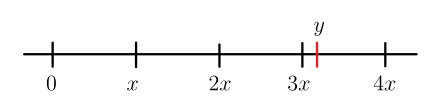
\includegraphics[scale=0.400]{Archimedisches_Prinzip.png}
\Satz[1.8] \newline
Für jedes \(t \geq 0, t \in \R\) hat \(x^2 = t\) eine Lösung in \(\R\) \newline
\Def[1.9] Seien \(x,y \in \R \) \newline
\begin{enumerate}
    \item [(i)] max\{x,y\} \(= \left\{\begin{array}{lll}
        x & \text { falls } & y \leq x \\
        y & \text { falls } & x \leq y
        \end{array}\right.\)
    \item[(ii)] min\{x,y\}  \(= \left\{\begin{array}{lll}
        y & \text { falls } & y \leq x \\
        x & \text { falls } & x \leq y
        \end{array}\right.\)
    \item[(iii)]  Der Absolutbetrag einer Zahl \(x \in \R: \newline \abs{x} = max\{x, -x\}\)
\end{enumerate}
\Satz[1.10]
\begin{enumerate}
    \item [(i)] \( \abs{x} \geq 0 \quad \forall x \in \R \)
    \item [(ii)] \(\abs{xy} = \abs{x}\abs{y} \quad \forall x,y \in \R \)
    \item [(iii)] \(\abs{x+ y} \leq \abs{x} + \abs{y} \quad \forall x,y \in \R\)
    \item [(iv)] \( \abs{x + y} \geq \abs{x} - \abs{y} \quad \forall x,y \in \R\)
\end{enumerate}
\Satz[1.11(Young'sche Ungleichung)] \newline
\(\forall \epsilon > 0, \forall x,y \in \R \):
\[2 \abs{xy} \leq \epsilon x^2 + \frac{1}{\epsilon}y^2\]
\sep
\subsection{Infimum und Supremum}
\Def[1.12]  Sei \(A \subseteq \R\) eine Teilmenge.
\begin{enumerate}
\item[1)]  \(c \in \R\) ist \textbf{obere Schranke} if  \(\forall a \in A: a \leq c\)
\item[2)]  \(c \in \R\) ist \textbf{untere Schranke} if \(\forall a \in A: c \leq a\)
\item[3)] \(m \in \R\) heisst ein \textbf{Maximum} von A if \(m \in A\) und \(m\) eine obere Schranke von A ist.
\item[4)] \(m \in \R\) heisst ein \textbf{Minimum} von A if \(m \in A\) und \(m\) eine untere Schranke von A ist.
\end{enumerate}

\Satz[1.15]. Sei \(A \subseteq \R, A \neq \emptyset\)
\begin{enumerate}
\item[1)]  Sei A nach oben beschränkt. Dann gibt es eine kleinste obere Schranke: 
\[c:=\sup A \text{ \ \textbf{(Supremum von A)}}\]
\item[2)]  Sei A nach unten beschränkt. Dann gibt es eine grösste untere Schranke: 
\[d:=\inf A \text{ \ \textbf{(Infimum von A)}} \]  
\end{enumerate}

Eigenschaften von Supremum und Infimum
\begin{enumerate}
\item[\(\bullet\)]  \(\sup (A \cup B) = \text{max} (\sup A, \sup B)\)
\item[\(\bullet\)]  \(\sup (A + B) = \sup A + \sup B\)
\item[\(\bullet\)]  \(\inf (A \cup B) = \text{min} (\inf A, \inf B)\)
\item[\(\bullet\)]  \(\inf (A + B) = \inf A + \inf B\)
\end{enumerate}
\Korollar[1.16]  Seien \(A \subseteq B \subseteq \R\) Teilmengen von \(\R\)
\begin{enumerate}
    \item [1] Falls B nach oben beschränkt ist, \newline \(\sup A \leq \sup B\)
    \item [2] Falls B nach unten beschränkt ist, \newline\(\inf B \leq \inf A\)
\end{enumerate}
\Bsp[1.17]
\begin{enumerate}
    \item \( A = [1,2[: sup A = 2, inf A = 1\)
    \item \( A = \sum_{k=1}^n \frac{1}{k} = 1 + \frac{1}{2}+ \dots + \frac{1}{n}\) ist nicht nacht oben beschränkt (harmonische Reihe)
    \item \( A = \{ 1 - \frac{1}{3},(1 - \frac{1}{3})+(\frac{1}{5}-\frac{1}{7}),(1 - \frac{1}{3})+(\frac{1}{5}-\frac{1}{7})+(\frac{1}{9}-\frac{1}{11}), \dots \}\)
    Dann gilt: \( \sup A = \frac{\pi}{4}\)(Leibniz).
\end{enumerate}

\sep
\Def[1.18] Kardinalität
\begin{enumerate}
    \item [(i)] Zwei Mengen X,Y heissen gleichmächtig if eine Bijection \(f: X \rightarrow Y\) existiert
    \item [(ii)] Eine Menge ist endlich, wenn \(X = \emptyset\) or \(\exists n \in \N\) so dass\(\{1,2,\dots,n\}\)gleichmächtig wie X
    \item [(iii)] Eine Menge X ist abzähbar if endlich oder gleichmächtig wie \(\N\)
\end{enumerate}
\Satz[1.20] (Cantor) \(\R\) ist nicht abzählbar

\sep
\section{Folgen und Reihen}
\Def[2.1] Eine \textbf{Folge} ist eine Abbildung 
\[a: \N^* \rightarrow \R (\N^* = \N / \{0\})\]
\sep
\subsection{Grenzwert einer Folge}
\Lemma[2.3]\((a_n)_{n\geq1}\) eine Folge, es gibt höchstens eine Zahl \(l \in \R\) mit der Eigenschaft: \newline
\(\forall \epsilon > 0\) ist Menge \(\{n \in \N : a_n \notin ]l-\epsilon, l+\epsilon [\}\) endlich \newline
\Def[2.4] \((a_n)_{n\geq1}\) ist \textbf{konvergent}, falls \(l \in \R\) so dass \(\forall \epsilon > 0\)
die Menge \(\{n \in \N^* : a_n \notin ]l-\epsilon, l+\epsilon [\}\) endlich ist. Dieses l ist der \textbf{Limes} der Folge. \newline
\Bem[2.5] Jede Konvergente Folge ist beschränkt
\Lemma[2.6] Folgende Aussagen sind äquivalent
\begin{enumerate}
    \item [1]  \((a_n)_{n\geq1}\) konvergiert gegen \(l = \lim\limits_{n \rightarrow \infty} a_n\)
    \item [2] \(\forall \epsilon > 0 \ \exists N \geq 1\) that
    \[ \abs{a_n - l} < \epsilon \quad \forall n \geq N \]
\end{enumerate}
\Bsp[2.7] Sei \( a_n = \frac{n}{n+1}, n \geq 1\). \newline Dann gilt: \( \lim_{n \rightarrow \infty} a_n = 1\) \newline
Begründung: \( a_n -1 = \frac{n}{n+1}-1 = \frac{-1}{n+1 }\). Es folgt \( \abs{a_n -1} = \frac{1}{n+1}\)
Sei \(  \epsilon > 0;\) Nach Archimedes gibt es \( N \in \N \) mit \( \frac{1}{N+1} < \epsilon \). \newline
Dann folgt \( \forall n \geq N\):
\[ \abs{a_n-1} = \frac{1}{n+1} \leq \frac{1}{N+1} < \epsilon \]
\Satz[2.8] Seien \((a_n)_{n \geq 1}\) und \((b_n)_{n \geq 1}\) konvergent Folgen mit \(a= \lim\limits_{n \rightarrow \infty} a_n\), $b = \lim\limits_{n \rightarrow \infty} b_n$
\begin{enumerate} 
    \item [1] \((a_n + b_n)_{n \geq 1}\) ist konvergent und \newline \(\lim\limits_{n \rightarrow \infty} (a_n + b_n) = a+b\)
    \item [2] \((a_n \cdot b_n)_{n \geq 1}\) ist konvergent und \newline \(\lim\limits_{n \rightarrow \infty} (a_n \cdot b_n) = a \cdot b\)
    \item [3] if \(b_n \neq 0 \ \forall n \geq 1, b \neq 0 \ (\frac{a_n}{b_n})_{n\geq 1}\) konvergent, \(\lim\limits_{n \rightarrow \infty} (\frac{a_n}{b_n}) = \frac{a}{b}\)
    \item [4] Falls existiert K \(\geq 1\) mit \(a_n \leq b_n \ \forall n \geq K \implies a \leq b\)
\end{enumerate}
\Bsp[2.9] \( b \in \Z: \lim_{n \rightarrow \infty } \left( 1 + \frac{1}{n}\right)^b = 1\) \newline
Das folgt aus \( \lim_{n \rightarrow \infty } \left( 1 + \frac{1}{n}\right) = 1 \) und wiederholter Anwendung von Satz 2.8 (2) \& (3)
\sep
\subsection{Satz von Weierstrass}
\Def[2.10]
\begin{enumerate}
    \item [1] \((a_n)_{n \geq 1}\) ist \textbf{monoton wachsend} if
    \[a_n \leq a_{n+1} \ \forall n \geq 1\]
    \item [2] \((a_n)_{n \geq 1}\) ist \textbf{monoton fallend} if 
    \[a_{n+1} \leq a_n \ \forall n \geq 1\]
    \newline
    \newline
\end{enumerate}

\Satz[2.11] (Weierstrass)
\begin{enumerate}
    \item [\(\bullet\)] Sei \((a_n)_{n \geq 1}\) monoton wachsend und nach oben beschränkt. Dann konvergiert \((a_n)_{n \geq 1}\) nach \[\lim\limits_{n \rightarrow \infty} a_n = \sup\{a_n : n \geq 1\}\]
    \item [\(\bullet\)] Sei \((a_n)_{n \geq 1}\) monoton fallend und nach unten beschränkt. Dann konvergiert \((a_n)_{n \geq 1}\) nach \[\lim\limits_{n \rightarrow \infty} a_n = \inf\{a_n : n \geq 1\}\]
\end{enumerate}
\Bsp[2.12] Sei \( a \in \Z\) und \( 0 \leq q < 1\). Dann gilt \( \lim_{n \rightarrow \infty} n^a q^n = 0\).
Sei \( x_n = n^a q^n\) dann folgt
\[ x_{n+1} = (n+1)^a q^{n+1} = \left( \frac{n+1}{n}\right)^a q \cdot n^a q^n =\] 
\[\left( 1 + \frac{1}{n}\right)^a \cdot q \cdot x_n\] Also:
\[ x_{n+1} = \left( 1 + \frac{1}{n}\right)^a \cdot q \cdot x_n\]
Da \( \lim_{n \rightarrow \infty} \left( 1 + \frac{1}{n}\right)^a = 1\) gibt es ein \(n_0\), so dass \( \left( 1 + \frac{1}{n}\right)^a < \frac{1}{q} \ \forall n \geq n_0\). Es folgt:
Da \( x_n > 0 \ \forall n \geq 1\) ist die Folge nach unten beschränkt und für \( n \geq n_0\) monoton fallend. Sei
\[ l = \lim_{ n \rightarrow \infty} x_n = \lim_{n \rightarrow \infty} x_{n+1} = \lim_{n \rightarrow \infty} \left( 1 + \frac{1}{n}\right)^a \cdot qx_n \] 
\[= q \cdot \lim_{n \rightarrow \infty} x_n = q \cdot l\]
Also \( (1-q) \cdot l = 0\) woraus l=0 folgt. \newline
\Bem[2.13] Oben haben wir folgede Tatsache benützt: Sei \( (a_n)_{n \geq 1}\) eine konvergente Folge mit \( \lim_{n \rightarrow \infty} a_n = a\) und \(k \in \N\). Dann ist die durch
\[b_n:= a_{n+k} \quad n \geq 1\]
definierte Folge konvergent und
\[ lim_{n \rightarrow \infty} b_n = a\]
\Bsp[2.14] \( \lim_{n \rightarrow \infty} \sqrt[n]{n} = 1\) \newline
\Bsp[2.15] Die Folge \( \left( 1 + \frac{1}{n}\right)^n, n \geq 1\) konvergiert. Der Limes ist
\[ e = \lim_{n \rightarrow \infty } \left( 1 + \frac{1}{n} \right)^n\]
die Eulersche Konstante \( e \approx 2.71828\)
\Lemma[2.16 (Bernoulli Ungleichung)]
\[(1+x)^n \geq 1 + n \cdot x \quad \forall n \in \N, x > -1\]
\Bsp[2.17] Sei \( c > 1\). Wir definieren \( (a_n)_{n \geq 1}\) durch:
\[ a_1 = c, \quad a_{n+1} = \frac{1}{2} \left( a_n + \frac{c}{a_n}\right) \quad n \geq 1\]
Dann existiert \( a:= \lim_{n \rightarrow \infty} a_n > 0\) und es gilt \( a^2 = c\)
\begin{enumerate}
    \item \( (a_n)_{n \geq 1}\) ist monoton fallend.
    \[ a_{n+1} = a_n + \frac{1}{2} \left( \frac{c}{a_n} - a_n\right) = a_n + \left( \frac{c - a_{n}^2}{2a_n}\right)\]
    Wir zeigen zunächst: \( a_n^2 \geq c \quad \forall n \geq 1\)
    Für \( n = 1: a_1^2 = c^2 > c\), da \( c > 1\). Und für \( n \geq 1\):
    \[ a_{n+1}^2 = a_n^2 + (c - a_n^2) + \left( \frac{c - a_n^2}{2 a_n}\right)^2 = \]
    \[ c + \left( \frac{c - a_n^2}{2 a_n}\right)^2 \geq c\]
    Aus \( a_n^2 \geq c \) folgt:
    \[ a_{n+1} = a_n + \left( \frac{c - a_n^2}{2 a_n }\right) \leq a_n \]
    \item Es ist klar: \( a_n > 0 \quad \forall n \geq 1\)
    Aus \( a_n^2 \geq c > 1\) folgt dann \( a_n \geq 1 \ \forall n \geq 1\)
    \item Nach Weierstrass: \( a = \lim_{n \rightarrow \infty } a_n\), dann folgt aus (2) \( a \geq 1 \& a \neq 0\)
    \[ a = \lim_{n \rightarrow \infty} a_{n+1} = \frac{1}{2} \left(\lim_{ n \rightarrow \infty } a_n + \frac{c}{\lim_{n \rightarrow \infty a_n}} \right)\] 
    \[= \frac{1}{2} \left( a + \frac{c}{a}\right) \implies a^2 = c\]
\end{enumerate}
\sep

\subsection{Limes inferior, Limes superior}
Eine wichtige Anwendung des Satzes von Weierstrass ist, wie man mit jeder beschränkten Folge \( (a_n)_{n \geq 1}\) zwei monotone Folgen \( (b_n)_{n \geq 1}\) und \( (c_n)_{n \geq 1}\) definieren kann, welche dann einen Grenzwert besitzen.

\[\lim\limits_{n \rightarrow \infty} \inf a_n = \lim\limits_{n \rightarrow \infty} b_n, (b_n = inf \{a_k : k \geq n\})\]


\[\lim\limits_{n \rightarrow \infty} \sup a_n = \lim\limits_{n \rightarrow \infty} c_n, \ (c_n = sup \{a_k : k \geq n\})\]
\[\lim\limits_{n \rightarrow \infty} \inf a_n \leq \lim\limits_{n \rightarrow \infty} \sup a_n\]
\Bsp[2.18] \( a_n = (-1)^n + \frac{1}{n}, \ n \geq 1\). \newline
Dann: \( b_n = -1\) und \( c_n = 1 + \frac{1}{n_g}\) wobei \( n_g\) die kleinste gerade Zahl \( \geq n\) bezeichnet. Also: \newline
\(\lim\limits_{n \rightarrow \infty} \inf a_n = -1 \) und \(\lim\limits_{n \rightarrow \infty} \sup a_n = +1\)
\sep
\subsection{Cauchy Kriterium}
Wie sieht man einer Folge an, ob sie konvergent ist, ohne ihren Grenzwert zu kennen? Dafür wird das Cauchy Kriterium angewendet. \newline
\Lemma[2.19] \((a_n)_{n \geq 1}\) konvergiert if only if \((a_n)_{n \geq 1}\) beschränkt und \[\lim\limits_{n \rightarrow \infty} \inf a_n = \lim\limits_{n \rightarrow \infty} \sup a_n\] 
\Satz[2.20 (Cauchy Kriterium)]. \newline Die Folge \((a_n)_{n \geq 1}\) ist genau dann konvergent wenn \[\forall \epsilon > 0 \ \exists N \geq 1 \  \text{so dass} \abs{a_n - a_m} < \epsilon \ \forall n,m \geq N\]
\sep
\subsection{Satz von Bolzano-Weierstrass}
In diesem Abschnitt zeigen wir, dass jede beschränkte Folge eine konvergente Teilfolge besitzt.
\Def[2.21] Ein abgeschlossenes Intervall ist \(I \subseteq \R\)
\begin{enumerate}
    \item [1] \([a,b] \quad a \leq b,\  a,b \in \R\)
    \item [2] \([a,+\infty[$ $a \in \R\)
    \item [3] \(]-\infty,a]$ $a \in \R\)
    \item [4] \(]-\infty,+\infty[ = \R\)
\end{enumerate}
Länge \(\mathcal{L}(I)\) ist in 1) $b-a$, ansonsten $+\infty$ \newline
\Bem[2.22] $I \subseteq \R$ ist abgeschlossen if only if für jede konvergente Folge \((a_n)_{n \geq 1}\) aus Elementen in I, der Grenzwert auch in I ist. \newline
\Bem[2.23] Seien \( I = [a,b], J = [c,d]\) mit \(a \leq b \) und \(c \leq d \ a,b,c,d \in \R\). Dann gilt \( I \subseteq J \) genau dann, wenn \(c \leq a \) und \(b \leq d\) \newline \newline \newline
\Satz[2.25 (Cauchy-Cantor)] Sei \(I_1 \supseteq I_2 \supseteq \dots\) eine Folge abgeschlossener Intervale mit \(\mathcal{L}(I_1) < +\infty\)
Dann gilt \[ {\bigcap}_{n\geq1} I_{n} \neq \emptyset \] Falls zudem \(\lim\limits_{n \rightarrow \infty} \mathcal{L}(I_n) = 0\) enthält \({\bigcap}_{n\geq1} I_{n}\) genau einen Punkt \newline
\Def[2.27] Eine Teilfolge einer Folge \((a_n)_{n \geq 1}\) ist eine Folge \((b_n)_{n \geq 1}\) wobei \[b_n = a_l(n)\] und \(l: \N^* \rightarrow \N^*\) eine Abbildung ist mit \[l(n) < l(n+1) \quad \forall n \geq 1s\] 
\Satz[2.29 (Bolzano.Weierstrass)] Jede beschränkte Folge besitzt eine Konvergente Teilfolge \newline
\Bem[2.30] Sei \((a_n)_{n \geq 1}\) eine beschränkte Folge. Dann gilt für jede konvergente Teilfolge \((b_n)_{n \geq 1} :\) \[\lim\limits_{n \rightarrow \infty} \inf a_n \leq \lim\limits_{n \rightarrow \infty} b_n \leq \lim\limits_{n \rightarrow \infty} \sup a_n\].
\sep
\subsection{Folgen in \(\R^{d}\) und \(\C\)}
\Def[2.31] Eine Folge in \(\R^d\) ist eine Abbildung \[a : \N^* \rightarrow \R^d\] 
\Def[2.32] Eine Folge \((a_n)_{n \geq 1}\) in \(\R^d\) heisst \textbf{konvergent}, falls es \(a \in \R^d\) gibt so dass: \[\forall \epsilon > 0 \  \exists N \geq 1 \ \text{mit} \ \abs{\abs{a_n-a}} < \epsilon \  \forall n \geq N\]
\Satz[2.33] Sei \(b = b_1, \dots , b_d\). 1) und 2) sind äquivalent: 
\begin{enumerate}
    \item [1] \(\lim\limits_{n \rightarrow \infty} a_n = b\)
    \item [2] \(\lim\limits_{n \rightarrow \infty} a_{n,j} = b_j \quad \forall 1 \leq j \leq d\)
\end{enumerate}
\Satz[2.36]
\begin{enumerate}
    \item [1] Eine Folge \((a_n)_{n \geq 1}\) konvergiert genau, wenn sie eine Cauchy Folge ist : \[\forall \epsilon > 0 \ \exists N \geq 1 \ \text{mit} \ \abs{\abs{a_n - a_m}} < \epsilon \  \forall n,m \geq N\]
    \item [2] Jede beschränkte Folge hat eine konvergente Teilfolge
\end{enumerate}
\sep
\subsection{Reihen}
\Def[2.7.0] Eine Reihe ist eine unendliche Summe
\[S_{n} := a_{1}  + \cdots + a_{n} = \sum_{k=1}^{n} a_{k}\]
\Def[2.37] Die Reihe \[\sum_{k=1}^{\infty} a_{k}\] ist \textbf{konvergent}, falls die Folge \((S_n)_{n \geq 1}\) der Partialsummen konvergiert. In diesem Fall : \[\sum_{k=1}^{\infty} a_{k} := \lim\limits_{n \rightarrow \infty} S_n\]
\Bsp[2.38](Geometrische Reihe). Sei \( q \in \C \) mit \( \abs{q} < 1\). Dann konvergiert \( \sum_{k=0}^{\infty} q^k \) und der Wert ist:
\[ \sum_{k=0}^{\infty} q^k = \frac{1}{1-q}\]
Sei \( S_n = \sum_{k=0}^n q^k = 1 + q + \dots + q^n\)
\[ q \cdot S_n = q + \dots q^n + q^{n+1}\]
woraus
\[(1-q)S_n = 1 - q^{n+1}\]
folgt. Es gilt also: \( S_n = \frac{1 - q^{n+1}}{1 - q}\) \newline
Nun zeigen wir die Konvergenz:
\[ \abs{S_n - \frac{1}{1-q}} = \abs{\frac{-q^{n+1}}{1-q}}= \frac{\abs{q}^{n+1}}{\abs{1-q}}\]
Aus Bsp 2.12 und \( 0 \leq \abs{q} < 1\) folgt:
\[ \lim_{n \rightarrow \infty} \abs{S_n-\frac{1}{1-q}} = \lim_{n \rightarrow \infty} \frac{\abs{q}^{n+1}}{\abs{1-q}} =0\]
Somit konvergiert \( (S_n)_{n \geq 1} \) gegen \( \frac{1}{1-q}\)
\Satz[2.40] Seien \(\sum_{k=1}^{\infty} a_{k}\) und \(\sum_{j=1}^{\infty} b_{j}\) konvergent, sowie \(\alpha \in \C \)
\begin{enumerate}
    \item [1] \(\sum_{k=1}^{\infty} (a_k + b_k)\) konvergent und \newline \(\sum_{k=1}^{\infty} (a_k + b_k) = (\sum_{k=1}^{\infty} a_{k}) + (\sum_{j=1}^{\infty} b_{j})\)
    \item [2] \(\sum_{k=1}^{\infty} \alpha \cdot a_k\) konvergent und \newline \(\sum_{k=1}^{\infty} \alpha \cdot a_k = \alpha \cdot \sum_{k=1}^{\infty}  a_k\)
\end{enumerate}
\sep
\Satz[2.41 (\textbf{Cauchy Kriterium})]  \newline Die Reihe \(\sum_{k=1}^{\infty} a_k \) konvergiert genau dann, wenn:
\[ \forall \epsilon > 0 \ \exists N \geq 1 \ \text{mit} \abs{\sum_{k=n}^{m} a_k} < \epsilon \quad \forall m \geq n \geq N\]
Anmerkung: Aus dem Cauchy Kriterium folgt das Nullfolgenkriterium.
Bildet die Folge der Summanden einer Reihe keine Nullfolge, dann divergiert die Reihe.
Also falls \( \lim_{n \rightarrow \infty} \abs{a_n} \neq 0 \implies \sum_{n=0}^\infty a_n \) divergiert. \newline
\Satz[2.42] Sei \(\sum_{k=1}^{\infty} a_{k}\) eine Reihe mit \newline \(a_k \geq 0 \quad \forall k \in \N^*\). Die Reihe \(\sum_{k=1}^{\infty} a_{k}\) konvergiert if only if \((S_n)_{n \geq 1}, S_n = \sum_{k=1}^{n} a_{k}\) der Partialsummen nach oben beschränkt ist. \newline
\sep
\Korollar[2.43 (\textbf{Vergleichssatz})] \newline Seien $\sum_{k=1}^{\infty} a_{k}$ und $\sum_{k=1}^{\infty} b_{k}$ Reihen mit: \[0 \leq a_{k} \leq b_{k} \quad \forall k \geq 1\]
\[ \sum_{k=1}^{\infty} b_{k} \text{ konvergent} \implies \sum_{k=1}^{\infty} a_{k} \text{ konvergent} \]
\[ \sum_{k=1}^{\infty} a_{k} \text{ divergent} \implies \sum_{k=1}^{\infty} b_{k} \text{ divergent} \]
Diese Implikation gilt auch, wenn \[K \geq 1 \  \text{mit} \ 0 \leq a_k \leq b_k \quad \forall k \geq K\]
\Bsp[2.44] \( \sum_{k=1}^\infty \frac{1}{k^2}\) konvergiert. \newline
Sei \( a_k = \frac{1}{k^2}, b_k = \frac{1}{(k-1)k},\  k \geq 1\). Dann gilt \( 0 \leq a_k \leq b_k, k \geq 2\) und
\[ \sum_{k=2}^{n}b_k = \sum_{k=2}^n\left( \frac{1}{k-1}- \frac{1}{k}\right) = \dots \left(\frac{1}{n-1} - \frac{1}{n}\right)\]
\[ = 1 - \frac{1}{n} < 1 \quad \forall n \geq 1\]
\sep
\Def[2.45] Die Reihe \(\sum_{k=1}^{\infty} a_{k}\) heisst \textbf{absolut konvergent}
\[\text{falls} \sum_{k=1}^{\infty} \abs{a_{k}} \text{konvergiert}\] \newline
\Satz[2.46] Eine absolut konvergente Reihe  \(\sum_{k=1}^{\infty} a_{k}\) ist auch konvergent und:
\[\abs{\sum_{k=1}^{\infty} a_{k}} \leq \sum_{k=1}^{\infty} \abs{a_{k}}\] \newline
\Bsp[2.47] \( \sum_{k=1}^\infty(-1)^{k+1} \frac{1}{k} \) konvergiert, ist aber nicht absolut konvergent.
\Satz[2.48 (Leibniz 1682)] Sei \((a_n)_{n \geq 1}\) monoton fallend mit \(a_n \geq 0 \quad \forall n \geq 1\) und \(\lim\limits_{n \rightarrow \infty} a_n = 0\). Dann konvergiert
\[S := \sum_{k=1}^{\infty} (-1)^{k+1}a_k \text{und es gilt} \  a_1 - a_2 \leq S \leq a_1\]
\Bsp[2.49] Betrachten wir nochmals Bsp 2.47
\[ S = 1 - \frac{1}{2} + \frac{1}{3} - \frac{1}{4} + \dots\]
\[ \frac{1}{2} = 1 - \frac{1}{2} \leq S \leq 1\]
\Def[2.50] Eine Reihe \(\sum_{n=1}^{\infty} a'_n\) ist eine \textbf{Umordnung} der Reihe \(\sum_{n=1}^{\infty} a_n\), falls eine bijektive Abbildung
\[\phi : \N^{*} \rightarrow \N^{*} \text{mit} \ a'_{n} = a_{\phi(n)}\] \newline
\Satz[2.52](Dirichlet 1837) Falls \(\sum_{n=1}^{\infty} a_n\) absolut konvergiert, dann konvergiert jede Umordnung (oder auch Teilfolge) der Reihe und hat den selben Grenzwert
\sep
\Satz[2.53(Quotientenkriterium] \newline Sei \((a_n)_{n \geq 1}\) mit \(a_n \neq 0 \quad \forall n \geq 1 \).Falls
\[\limsup\limits_{n \rightarrow \infty} \frac{\left|a_{n+1}\right|}{\left|a_{n}\right|}<1 \implies \sum_{n=1}^{\infty} a_{n} \ \text{konvergiert absolut}\]
Falls
\[\liminf\limits_{n \rightarrow \infty} \frac{\left|a_{n+1}\right|}{\left|a_{n}\right|}>1 \implies \sum_{n=1}^{\infty} a_{n} \ \text{divergiert}\]
\Bsp[2.54](Exponentialfunktion). Für \( z \in \C \) betrachte die Reihe
\[ 1 + z \frac{z^2}{2!} + \frac{z^3}{3!} + \dots\]
mit allgemeinem Glied
\[ a_n = \frac{z^n}{n!}\]
Dann folgt für \( z \neq 0:\)
\[ \frac{\abs{a_{n+1}}}{\abs{a_n}} = \frac{\abs{z}}{n+1}\]
also gilt \( \lim_{n \rightarrow \infty} \frac{\abs{a_{n+1}}}{\abs{a_n}} = 0\)
und die Reihe konvergiert für alle \( z \in \C\) \newline
\Bem{2.55} Das Quotientenkriterium versagt, z.B wenn unendliche viele Glieder der Reihe verschwinden
\sep
\Satz[2.56 Wurzelkriterium]
\begin{enumerate}
    \item [1] Falls \[\limsup\limits_{n \rightarrow \infty} \sqrt[n]{\abs{a_n}} < 1\] dann konvergiert \(\sum_{n=1}^{\infty} a_n\) absolut
    \item [2] Falls \[\limsup\limits_{n \rightarrow \infty} \sqrt[n]{\abs{a_n}} > 1\] dann diviergiert \(\sum_{n=1}^{\infty} a_n\) und \(\sum_{n=1}^{\infty}\abs{a_n} \)
\end{enumerate}
\Def[Kovergenzradius]
Gibt den Bereich an, in welchem für eine Potenzreihe Konvergenz garantiert ist.
Sei \((c_k)_{k \geq 0} \) eine Folge in \( \R \) oder \( \C \). Falls \( \lim_{n \rightarrow \infty} \sup \sqrt[k]{\abs{c_k}}\) existiert, definieren wir
\begin{equation}
    \rho=\left\{\begin{array}{cc}
    +\infty \quad \quad \limsup _{k \rightarrow \infty} \sqrt[k]{\left|c_{k}\right|}=0 \\
    \frac{1}{\limsup _{k \rightarrow \infty} \sqrt[k]{\left|c_{k}\right|}} \limsup _{k \rightarrow \infty} \sqrt[k]{\left|c_{k}\right|}>0
    \end{array}\right.
    \end{equation}
Falls ab einem bestimmten Index all \(a_n \neq 0\) und der folge limes definiert ist, kann man den Konvergenzradius auch mit dem Quotientenkriterium ausrechen.
\[ \rho = \lim_{n \rightarrow \infty} \abs{\frac{a_n}{a_{n+1}}}\]
\Korollar[2.57] Die Potenzreihe \[\sum_{k=0}^{\infty} c_kz^k\]
\begin{itemize}
    \item konvergiert absolut für alle $\abs{z} < \rho$ 
    \item divergiert für alle $\abs{z} > \rho$
\end{itemize}
\Def[] Die Zeta Funktion
Sei \( s > 1\) und
\[ \zeta(s) = \sum_{n=1}^{\infty} \frac{1}{n^s}\]
Für \(s > 1\) konvergiert die obige Reihe
\Def[2.58] \(\sum_{k=0}^{\infty} b_k \) ist eine \textbf{lineare Anordnung} der Doppelreihe \(\sum_{i,j \geq 0} a_{i,j}\), falls es eine Bijektion \[\sigma : \N \rightarrow \N \times \N \] gibt mit \(b_k = a_{\sigma(k)}\) \newline
\Satz[2.59] (Cauchy 1821). Wir nehmen an, dass es \(B \geq 0\) gibt, so dass
\[\sum_{i=0}^{m}\sum_{j=0}^{m}\abs{a_{ij}} \leq B \quad \forall m \geq 0\]
Dann konvergieren die folgenden Reihen absolut:
\[S_i := \sum_{j=0}^\infty a_{ij} \quad \forall i \geq 0 \  \text{und} \  U_j := \sum_{i=0}^{\infty}a_{ij} \quad \forall j \geq 0\]
sowie
\[\sum_{i=0}^\infty S_i \ \text{und} \ \sum_{j=0}^\infty U_j\]
und es gilt:
\[\sum_{i=0}^\infty S_i  =  \sum_{j=0}^\infty U_j\]
Zudem konvergiert jede lineare Anordnung der Doppelreihe absolut, mit selbem Grenzwert \newline
\Def[2.60] Das \textbf{Cauchy Produkt} der Reihe
\[\sum_{i=0}^\infty\ a_i, \sum_{j=0}^\infty\ b_j\]
ist die Reihe
\[\sum_{n=0}^\infty ( \sum_{j=0}^n a_{n-j}b_j )= a_0b_0 + (a_0b_1 + a_1b_0) + \dots \] \newline
\Satz[2.62] Falls die Reihen
\[\sum_{i=0}^\infty a_i , \sum_{j=0}^\infty b_j\]
absolut konvergieren, so konvergiert ihr Cauchy Produkt und es gilt:
\[\sum_{n=0}^{\infty} (\sum_{j=0}^n a_{n-j}b_j) = (\sum_{i=0}^{\infty} a_i) (\sum_{j=0}^{\infty} b_j)\]
\Satz[2.64]  Sei \( f_n : \N \rightarrow \R \) eine Folge. Wir nehmen an :
\begin{enumerate}
    \item [1] \(f(j) := \lim\limits_{n \rightarrow \infty} f_n(j)\) existiert \(\forall j \in \N\)
    \item [2] Es gibt eine Funktion \(g: \N \rightarrow [0, \infty[\), so dass
    \begin {enumerate}
    \item [2.1] \(\abs{f_n(j)} \leq g(j) \quad \forall j \geq 0, \forall n \geq 0\)
    \item [2.2] \(\sum_{j=0}^\infty g(j)\) konvergiert
    \end{enumerate}
\end{enumerate}
Dann folgt
\[\sum_{j=0}^\infty f(j) = \lim\limits_{n \rightarrow \infty} \sum_{j=0}^\infty f_n(j)\]
\Korollar[2.65] Für jedes \(z \in \C \) konvergiert die Folge \(((1 + \frac{z}{n})^n)_{n \geq 1}\) und
\[\lim\limits_{n \rightarrow \infty} (1 + \frac{z}{n})^n = \exp(z)\]
\sep
\section{Stetige Funktionen}
\subsection{Reellwertige Funktionen}
\Def[3.1] Sei \( f \in \R^d\)
\begin{enumerate}
    \item [1] f ist nach \textbf{oben beschränkt}, if \(f(D) \subseteq \R \) nach oben beschränkt ist
    \item [2] f ist nach \textbf{unten beschränkt}, if \(f(D) \subseteq \R \) nach unten beschränkt ist
    \item [3] f ist beschränkt, if \(f(D) \subseteq \R \) b ist
\end{enumerate}
\Def[3.2] Eine funktion \(f: D \rightarrow \R\), wobei \(D \subseteq \R\) ist
\begin{enumerate}
    \item [1] \textbf{monoton wachsend}, if \(\forall x,y \in D\)
    \[x \leq y \implies f(x) \leq f(y) \]
    \item [2] \textbf{streng monoton wachsend}, if \(\forall x,y \in D\)
    \[x < y \implies f(x) < f(y)\]
    \item [3] \textbf{monoton fallend}, if \(\forall x,y \in D\)
    \[x \leq y \implies f(x) \geq f(y)\]
    \item [4] \textbf{streng monoton fallend}, if \(\forall x,y \in D\)
    \[x < y \implies f(x) > f(y)\]
    \item [5] \textbf{monoton}, falls f monoton wachsend oder monoton fallend
    \item [6] \textbf{streng monoton}, falls f streng monoton wachsend/fallend
\end{enumerate}
\sep
\subsection{Stetigkeit}
\Def[3.4] Sei \(D \subseteq \R, x_0 \in D\). Die Funktion \(f: D \rightarrow \R \) ist in \textbf{\(x_0\) stetig}, falls es für jedes \(\epsilon > 0 \) ein \(\delta > 0\) gibt, so dass für alle \(x \in D \) die Implikation
\[ \abs{x - x_0} < \delta \implies \abs{f(x) - f(x_0)} < \epsilon\] \newline
\Bsp[3.6] Sei \( n \geq 0: f: \R \rightarrow \R, x \rightarrow x^n\) ist stetig.
\hspace*{-5mm}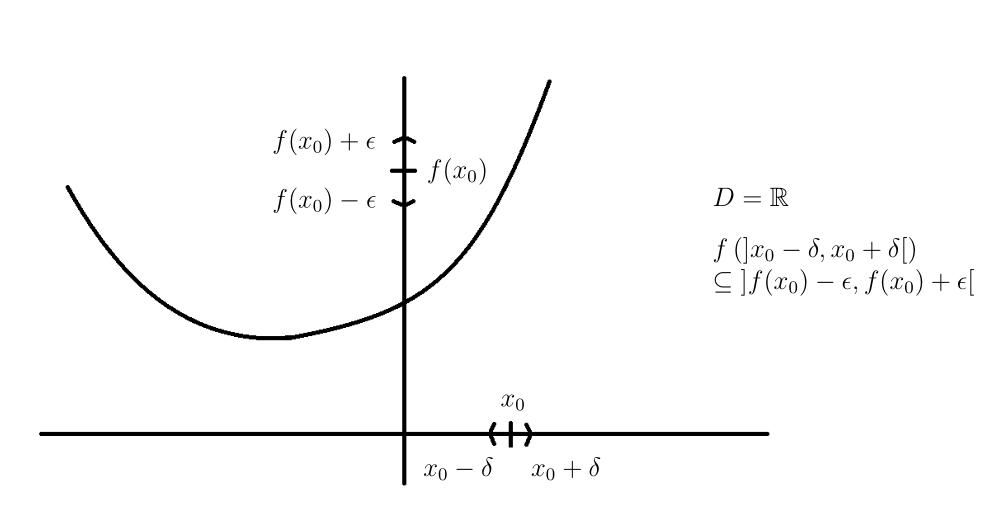
\includegraphics[scale=0.210]{Stetigkeit.png}
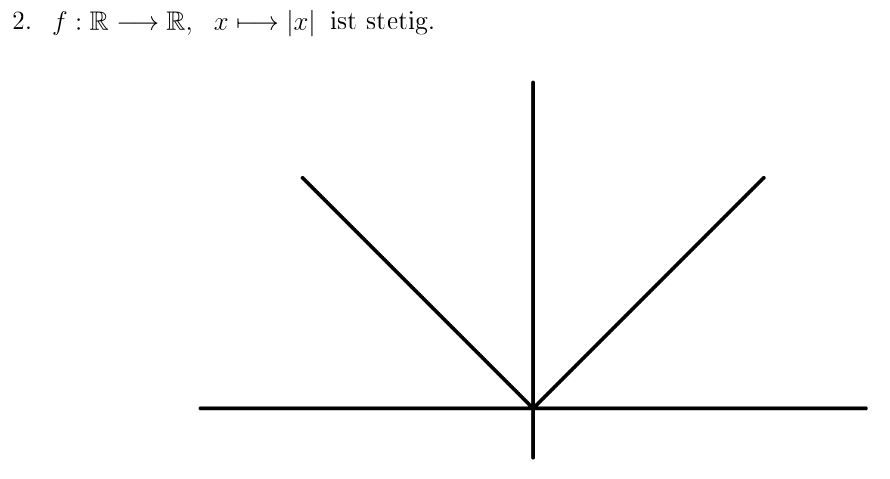
\includegraphics[scale=0.220]{Stetig2.png}
Die Abrundungsfunktion \( \lceil \cdot \rceil : \R \rightarrow \R, x \rightarrow \lceil x \rceil := \max \{ m \in \Z: m \leq z\}\)
ist in jedem Punkt \( x_0 \notin \Z \) stetig; sie ist in keinem Punkt \(y \in \Z \) stetig.
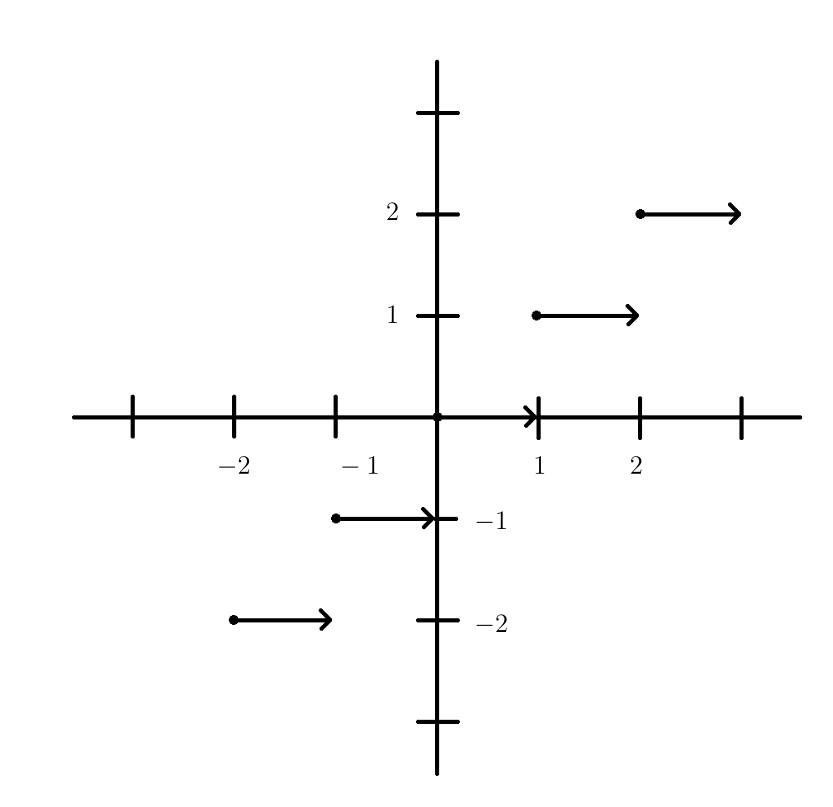
\includegraphics[scale=0.200]{Stetigkeit3.png}
Die Funktion \(f : \R \rightarrow \R \) definiert durch:

\Def[3.5] Die Funktion \(f : D \rightarrow \R\) ist \textbf{stetig}, falls sie in jedem Punkt von D stetig ist. \newline
\Satz[3.7] Sei \(x_0 \in D \subseteq \R \) und \(f: D \rightarrow \R \). Die Funktion f ist genau dann in \(x_0\) stetig falls für jede Folge \((a_n)_{n \geq 1}\) in D folgende implikation gilt:
\[\lim\limits_{n \rightarrow \infty} a_n = x_0 \implies \lim\limits_{n \rightarrow \infty} f(a_n) = f(x_0)\]
\Korollar[3.8] Sei \(x_0 \in D \subseteq \R, \lambda \in \R \) und \(f : D \rightarrow \R, \) \newline \( g: D \rightarrow \R\) beide stetig in \(x_0\)
\begin{enumerate}
    \item [1] Dann sind \(f+g, \lambda \cdot f, f \cdot g\) stetig in \(x_0\)
    \item [2] Falls \(g(x_0) \neq 0\) dann ist
    \[ \frac{f}{g} : D \cap \{x \in D : g(x) \neq 0\} \rightarrow \R\]
    \[x \rightarrow \frac{f(x)}{g(x)}\] stetig in \(x_0\)
\end{enumerate}
\Def[3.9] Eine \textbf{polynomiale Funktion} \(P: \R \rightarrow \R\) ist eine Funktion der Form
\[P(x) = a_nx^n + \dots + a_0\]
wobei : \(a_n \dots a_0 \in \R\). Falls \(a_n \neq 0\) ist n der \textbf{Grad} von P \newline
\Korollar[3.10] Polynomiale Funktionen sind auf ganz \(\R\) stetig \newline
\Korollar[3.11] Seien P,Q, polynomiale Funktionen auf \(\R\) mit \(Q \neq 0\). Seien \(x_1 \dots x_m\) die Nullstellen von Q. Dann ist
\[\frac{P}{Q} : \R \setminus \{x_1, \dots x_m\} \rightarrow \R \]
\[x \rightarrow \frac{P(x)}{Q(x)}\] stetig
\sep
\subsection{Der Zwischenwertsatz}
\Satz[3.12] (Bolzano 1817). Sei \(I \subseteq \R \) ein Intervall, \(f : I \rightarrow \R \) eine stetige Funktion und \(a,b \in I\). Für jedes \(c\) zwischen \(f(a)\) und \(f(b)\) gibt es ein \(z\) zwischen a und b mit \(f(z) = c\) \newline
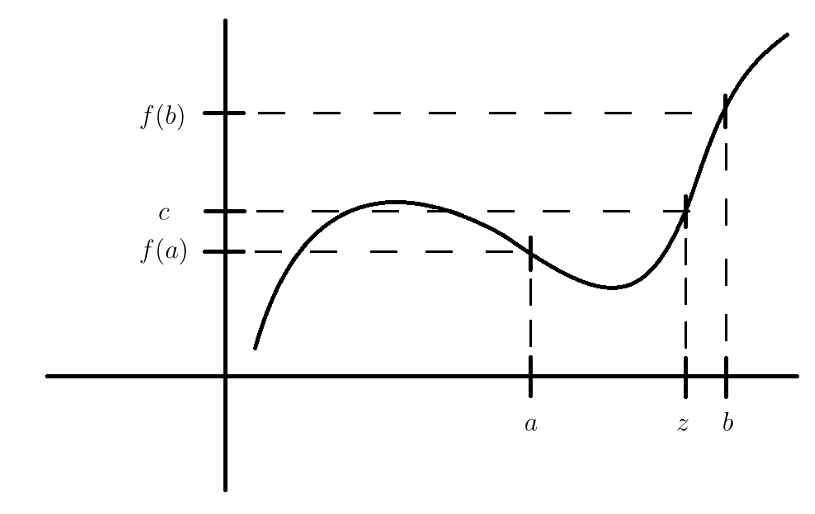
\includegraphics[scale=0.200]{Zwischenwertsatz.png}
\Korollar[3.13] Sei \(P(x) = a_nx^n + a_{n-1}x^{n-1} + \dots + a_0\) ein Polynom mit \(a_n \neq 0\) und \(n\) ungerade. Dann besitzt P mindestens eine Nullstelle in \(\R\) \newline
\Bem[3.14] für \(c > 0\) besitzt \(Q(x) = x^2 + c\) keine Nullstelle in \(R\) \newline
\sep
\subsection{Der Min-Max Satz}
In diesem Abschnitt zeigen wir, dass eine stetige Funktion auf einem kompakten Intervall beschränkt ist und zudem ein Maximum und ein Minimum annimmt.
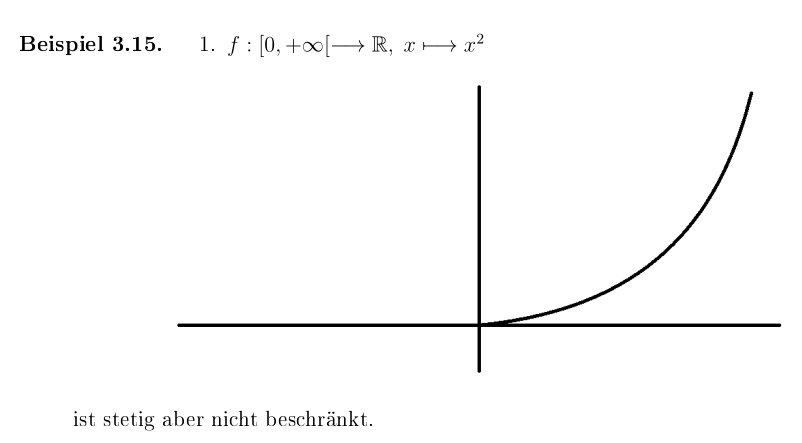
\includegraphics[scale=0.255]{3.151.png}
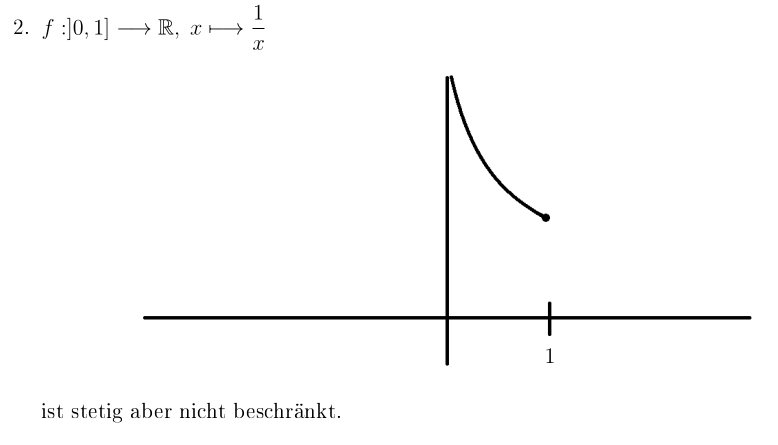
\includegraphics[scale=0.255]{3.152.png}
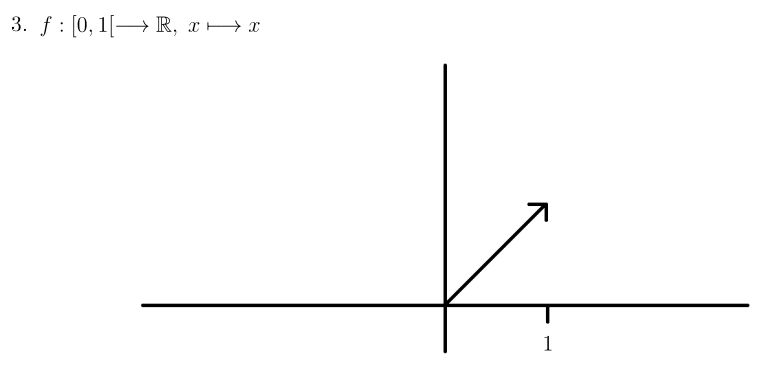
\includegraphics[scale=0.255]{3.153.png}
wobei das 3. Beispiel stetig und beschränkt ist, allerdings nimmt es kein Maximum an: Es gibt kein \( a \in [0,1[\), so dass \( f(x) \leq f(a) \quad \forall x \in [0,1[\)
\Def[3.16] Ein Intervall \(\subseteq \R\) ist \textbf{kompakt}, falls es von Form
\[I = [a.b], \quad a \leq b\] ist \newline
\Lemma[3.17] Sei \(D \subseteq \R, x_0 \in D \) und \(f,g : D \rightarrow \R \) stetig in \(x_0\). Dann sind
\[ \abs{f}, \max(f,g), \min(f,g) \] stetig in \(x_0\) \newline
\Lemma[3.18] Sei \((x_n)_{n \geq 1}\) eine konvergente Folge in \(\R\) mit Grenzwert
\[\lim\limits_{n \rightarrow \infty} x_n \in \R \]
sei \(a \leq b\). Falls \(\{x_n : n \geq 1\} \subseteq [a,b]\) folgt
\[\lim\limits_{n \rightarrow \infty} x_n \in [a,b] \]
\Satz[3.19] Sei \(f : I = [a,b] \rightarrow \R \) stetig auf dem kompakten Intervall I. Dann gibt es \(u \in I \) und \(v \in I\) mit
\[f(u) \leq f(x) \leq f(v) \quad \forall x \in I\]
Insbesondere ist f beschränkt
\sep
\subsection{Der Satz über  Umkehrabbildung} 
\Satz[3.20] Seien \(D_1, D_2 \subseteq \R \ zwei \ Teilmengen,\) \newline \(f: D_1 \rightarrow D_2, g: D_2 \rightarrow \R\) Funktionen, sowie \(x_0 \in D_1\). Falls \(f\) in \(x_0\) und \(g\) in \(f(x_0)\) stetig sind
\[ g \circ f : D_1 \rightarrow \R \]
in \(x_0\) stetig \newline
\Korollar[3.21] Falls in Satz 3.20 \(f\) auf \(D_1\) und \(g\) auf \(D_2\) stetig sind, so ist \(g \circ f\) auf \(D_1\) stetig \newline
\Satz[3.22] Sei \(I \subseteq \R\) ein Intervall und \(f: I \rightarrow \R\) stetig, streng monoton. Dann ist \(J:= f(I) \subseteq \R\) ein Intervall und \(f^{-1} : J \rightarrow I \) ist stetig. streng monoton. \newline
\Bsp[3.23] Sei \( n \geq 1\). Dann ist
\[ [0, \infty[ \rightarrow [0,\infty[ \]
\[ x \rightarrow x^n\]
streng monoton wachsend, stetig und surjektiv. Nach dem Umkehrsatz existiert eine streng monoton wachsende stetige Umkehrabbildung
\[ [0, \infty[ \rightarrow [0, \infty[\]
\[ x \rightarrow \sqrt[n]{x}\]
\sep
\subsection{Die reelle Exponentialfunktion}
\Def[Exponentialfunktion] \[ \exp(z) := \sum_{n=0}^{\infty} \frac{z^n}{n!} \quad z \in \R\]
\Satz[3.24] \(\exp: \R \rightarrow ]0,+\infty[\) ist streng monoton wachsend, stetig und surjektiv \newline
\Korollar[3.25] \[ \exp(x) > 0 \quad \forall x \in \R \]
\[\exp(x) > 1 \quad \forall x > 0\] \newline
\Korollar[3.26] \[\exp(z) > \exp(y) \quad \forall z > y\]
\Korollar[3.27] \[\exp(x) \geq 1 + x \quad \forall x \in \R\]
\Korollar[3.28] Der natürliche Logarithmus
\[\ln : ]0,+\infty[ \longrightarrow \R \] ist eine streng monoton wachsende, stetige, bijektive Funktion. Des Weiteren gilt:
\[\ln(a \cdot b) = \ln a + \ln b \quad \forall a,b \in ]0,+\infty[\]
Wir können den Logarithmus und die Exponentialfunktion benutzen, um allgemeine Potenzen zu definieren. Für \(x > 0\) und \( a \in \R \) beliebig definieren wir:
\[ x^a := \exp( a \ln x)\]
Insbesondere \( x^0 = 1 \quad \forall x > 0\) \newline
\Korollar[3.29]
\begin{enumerate}
    \item [1] Für \(a > 0\) ist \[]0,+\infty[ \longrightarrow ]0,+\infty[\]
    \[x \longrightarrow x^a\] eine stetige, streng monoton wachsende Bijektion \newline
    \item [2] Für \(a < 0\) ist \[]0,+\infty[ \longrightarrow ]0,+\infty[\]
    \[x \longrightarrow x^a\] eine stetige, streng monoton fallende Bijektion
    \item [3] \(ln(x^a) = a \ln(x) \quad \forall a \in \R, \forall x > 0\)
    \item [4] \(x^a \cdot x^b = x^{a+b} \quad \forall a,b \in \R, \forall x > 0\)
    \item [5] \((x^a)^b = x^{a \cdot b} \quad \forall a,b \in \R, \forall x > 0\)
\end{enumerate}
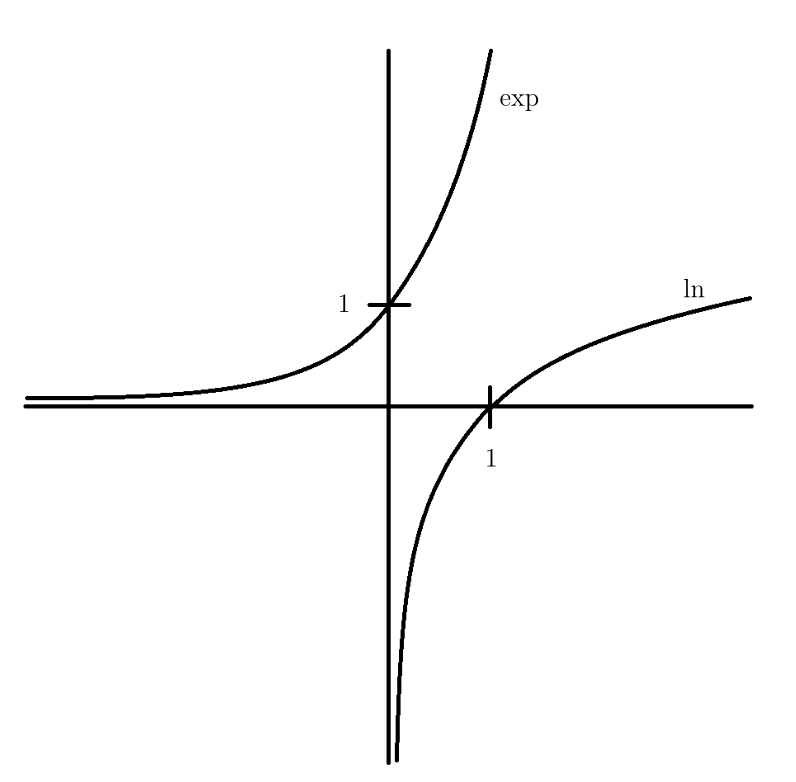
\includegraphics[scale=0.255]{lnExp.png}
\sep
\subsection{Konvergenz v. Funktionenfolgen}
Eine Funktionenfolge ist eine Abbildung 
\[ \N \longrightarrow \R^D\]
\[ n \longrightarrow f(n)\]
\Def[3.30] Die Funktionenfolge \((f_n)_{n \geq 0}\) \textbf{konvergiert punktweise} gegen eine Funktion \(f: D \rightarrow \R\), falls für alle \(x \in D :\)
\[f(x) = \lim\limits_{n \rightarrow \infty}f_n(x)\]
\Bsp[3.31] Sei \( D = [0,1]\) und
\[ f_n: [0,1] \rightarrow \R, \ n \in \N\]
\[ x \rightarrow x^n\]
Dann folgt aus Bsp 2.12
\[ lim_{n \rightarrow \infty} f_n(x) = \lim_{n \rightarrow \infty} x^n = 0 \quad \forall 0 \leq x < 1\]
Ausserdem gilt \( f_n(1) = 1^n = 1\). Also konvergiert die Funktonenfolge \( (f_n)_{n \geq 0}\) punktweise gegen die Funktion \( f:[0,1] \rightarrow \R\) gegeben durch:
\begin{equation}
f(x)=\left\{\begin{array}{lc}
0 & 0 \leq x<1 \\
1 & x=1
\end{array}\right.
\end{equation}
Bemerke: die Funktionen \(f_n\) sind alle stetig in \([0,1]\), die Funktion f ist nicht stetig in 1.
Um zu garantieren, dass der Grenzwert einer Folge stetiger Funktionen stetig ist, braucht es zusätzliche Voraussetzungen. \newline
\Def[3.32] (Weierstrass 1841) Die Folge
\[f_n : D \longrightarrow \R \]
\textbf{konvergiert gleichmässig} in D gegen
\[f : D  \rightarrow \R\]
falls gilt \( \forall \epsilon > 0 \quad \exists N \geq 1\), so dass
\[\forall n \geq N,\  \forall x \in D :\  \abs{f_n(x) - f(x) } < \epsilon \] \newline
In dieser Definition ist es wichtig, dass \(N\) nur von \( \epsilon\) abhängig ist und nicht von \(x \in D\).Deswegen kommt die Bedingung \(\forall x \in D\) nach der Bedingung \(\exists N \geq 1\)
\Satz[3.33] Sei \(D \subseteq \R\) und \(f_n : D \rightarrow \R \) eine Funktionenfolge bestehend aus(in D) stetigen Funktionen die (in D) gleichmässig gegen eine Funktion \(f: D \rightarrow \R \) konvergiert. Dann ist \(f\) (in D) stetig \newline
\Def[3.34] Eine Funktionenfolge
\[f_n : D \longrightarrow \R\]
ist \textbf{gleichmässig konvergent}, falls für alle \(x \in D\) der Grenzwert
\[f(x) := \lim\limits_{n \rightarrow \infty} f_n(x)\]
existiert und die Folge \((f_n)_{n \geq 0}\) gleichmässig gegen \(f\) konvergiert \newline
\Korollar[3.35] Die Funktionenfolge
\[f_n : D \longrightarrow \R \]
konvergiert genau dann gleichmässig in D, falls
\[\forall \epsilon > 0 \quad \exists N \geq 1 , \text{so dass} \  \forall n,m \geq N \ \text{und} \ \forall x \in D:\]  \newline
\[ \abs{f_n(x) - f_m(x)} < \epsilon \]
\Korollar[3.36] Sei \(D \subseteq \R\). Falls \(f_n : D \longrightarrow \R \) eine gleichmässig konvergente Folge stetiger Funktionen ist, dann ist die Funktion
\[f(x) := \lim\limits_{n \rightarrow \infty} f_n(x)\] stetig \newline
\Def[3.37] \(f_n: D \longrightarrow \R\) eine Folge von Funktionen. Die Reihe \(\sum_{k=0}^\infty f_k(x)\) konvergiert gleichmässig (in D), falls die durch
\[S_n(x) := \sum_{k=0}^{n}f_k(x)\] definierte Funktionenfolge gleichmässig konvergiert
\Satz[3.38] Sei \(D \subseteq \R \) und
\[f_n : D \rightarrow \R \]
eine Folge stetiger Funktionen. Wir nehmen an
\[\abs{f_n(x)} < c_n \quad \forall x \in D \]
und, dass \(\sum_{n=0}^\infty c_n\) konvergiert. Dann konvergiert die Reihe
\[\sum_{n=0}^\infty\ f_n(x)\]
gleichmässin in D und deren Grenzwert
\[f(x) := \sum_{n=0}^{\infty} f_n(x)\]
ist eine in D stetige Funktion \newline
\Def[3.39] Die Potenzreihe
\[\sum_{k=0}^\infty c_kx^k\]
hat \textbf{positiven Konvergenzradius}, falls \(\limsup\limits_{k \rightarrow \infty} \sqrt[k]{\abs{c_k}}\) existiert
Der Konvergenzradius ist dann definiert als:
\[\rho = \begin{cases}
    +\infty \quad \quad \quad \quad \quad \  \text{falls} \limsup_{k \rightarrow \infty} \sqrt[k]{\abs{c_k}} = 0 \\
    \frac{1}{\limsup\limits_{c \rightarrow \infty} \sqrt[k]{\left|c_{k}\right|}}  \quad \  \ \text{falls } \limsup_{k \rightarrow \infty} \sqrt[k]{\abs{c_k}} > 0
    \end{cases}\]
\newline
\Satz[3.40] Sei \(\sum_{k=0}^\infty c_kx^k \) eine Potenzreihe mit positivem Konvergenzradius \(\rho > 0\) und sei 
\[f(x) := \sum_{k=0}^\infty c_kx^k, \abs{x} < \rho \]
Dann gilt: \(\forall 0 \leq r < \rho \) konvergiert
\[\sum_{k=0}^\infty c_kx^k \]
gleichmässig auf \([-r,r]\), insbesondere ist \newline \(f: ] -\rho,\rho [ \longrightarrow \R\) stetig \newline
\sep
\subsection{Trigonometrische Funktionen}
\Def[Sinus\&Cosinus] \[ \sin(z) = z - \frac{z^3}{2!}+\frac{z^5}{5!}-\frac{z^7}{7!}+ \dots = \sum_{n=0}^{\infty} \frac{(-1)^nz^{2n+1}}{(2n)!}\]
\[ \cos(z) = 1-\frac{z^2}{2!}+\frac{z^4}{4!}-\frac{z^6}{6!}+\dots = \sum_{n=0}^{\infty} \frac{(-1)^nz^{2n}}{(2n)!}\]
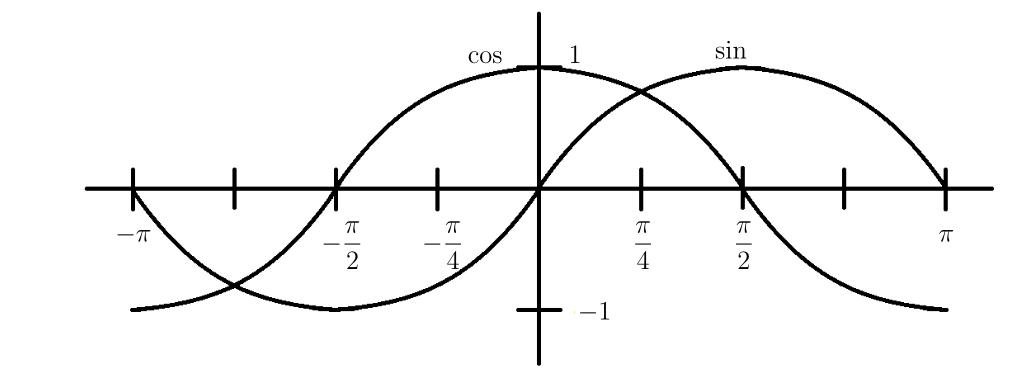
\includegraphics[scale=0.200]{SinCos.png}
\Satz[3.41] \( \sin: \R \rightarrow \R \) und \(\cos: \R \rightarrow \R \) sind stetige Funktionen \newline
\Satz[3.42]
\begin{enumerate}
    \item [1] \( \exp iz = \cos(z) + i \ sin(z) \quad \forall z \in \C \)
    \item [2] \( \cos(z) = \cos(-z)\) und \newline \(\sin(-z) = -\sin z \quad \forall z \in \C \)
    \item [3] \( \sin z = \frac{e^{iz} - e^{-iz}}{2i}, \cos z = \frac{e^{iz} - e^{-iz}}{2}\)
    \item [4] \( \sin(z + w) = \sin(z) \cos(w) + \cos(z) \sin(w)\) \newline
    \( \cos(z + w) = \cos(z) \cos(w) - \sin(z) \sin(w) \)
    \item [5] \( \cos(z)^2 + \sin(z)^2 = 1 \quad \forall z \in \C \)
\end{enumerate}
\Korollar[3.34]
\[\sin(2z) = 2 \sin(z) \cos(z)\]
\[\cos(2z) = \cos(z)^2 - \sin(z)^2\]
\sep
\subsection{Die Kreiszahl \( \pi \)}
\Satz[3.44] Die Sinusfuktion hat auf \(]0,+ \infty [\) mindestens eine Nullstelle
\[ \pi := \inf\{t > 0 : \sin t = 0\}\]
Dann gilt:
\begin{enumerate}
    \item [1] \( \sin \pi = 0,\quad \pi \in ]2,4[\)
    \item [2] \( \forall x \in ]0,\pi [: \sin x > 0\)
    \item [3] \( e^\frac{i \pi}{2} = i\)
\end{enumerate}
\Korollar[3.45]
\[ x \geq \sin x \geq x - \frac{x^3}{3!} \quad \forall 0 \leq x \leq \sqrt{6}\]
\Korollar[3.46]
\begin{enumerate}
    \item [1] \(e^{i \pi} = -1, \quad e^{2 i \pi} = 1\)
    \item [2] \( \sin(x + \frac{\pi}{2}) = \cos(x), \) \newline \(\cos(x + \frac{\pi}{2}) = -  \sin(x) \quad \forall x \in \R\)
    \item [3] \( \sin(x + \pi ) = - \sin(x), \) \newline \( \sin(x + 2 \pi) =  \sin(x) \quad \forall x \in \R \)
    \item [4] \( \cos (x + \pi) = - \cos(x), \) \newline \(\cos(x + 2 \pi) = \cos(x) \quad \forall x \in \R \)
    \item [5] Nullstellen von Sinus = \(\{ k \cdot \pi : k \in \Z\}\)
    \[ \sin(x) > 0 \quad \forall x \in ]2k \pi, (2k + 1) \pi [ ,\quad k \in \Z\]
    \[ \sin(x) < 0 \quad \forall x \in ](2k+1) \pi, (2k + 2) \pi [, \quad k \in \Z\]
    \item [6] Nullstellen von Cosinus \(= \{ \frac{\pi}{2} + k \cdot \pi : k \in \Z \}\)
    \( cos(x) > 0 \) \newline \(\quad \forall x \in ] -\frac{\pi}{2} + 2k \pi, -\frac{\pi}{2} + (2k+1) \pi [, \quad k \in \Z\)
    \( cos(x) < 0 \) \newline \(\forall x \in ] -\frac{\pi}{2} + (2k+1) \pi, -\frac{\pi}{2} + (2k + 2) \pi[,\quad k \in \Z\)
\end{enumerate}
Für \(z \notin \frac{\pi}{2} + \pi \cdot \Z \) definieren wir:
\[\tan(z) = \frac{\sin(z)}{\tan(z)}\]
und für \( z \notin \pi \cdot \Z\) :
\[\cot(z) = \frac{\cos(z)}{\sin(z)}\]
\sep
\subsection{Grenzwerte von Funktionen}
\Def[3.47] \(x_0 \in \R \) ist ein \textbf{Häufungspunkt} der Menge D falls \( \forall \delta > 0\) : 
\[ (]x_0 - \delta, x_0 + \delta [ \setminus \{x_0\}) \cap D \neq \emptyset \]
\Bsp[3.48] Sei \( D = \{0\} \cup ]1,2[.\) Dann ist die Menge \(D'\) der Häufungspunkt von D:
\[ D' =[1,2]\]
\Def[3.49] Sei \( f: D \longrightarrow \R, x_0 \in \R \) ein Häufungspunkt von D. Dann ist \(A \in \R \) der Grenzwert von \(f(x)\) für \(x \rightarrow x_0\) bezeichnet mit
\["\lim\limits_{x \rightarrow x_0} f(x) = A"\]
falls \( \forall \epsilon > 0 \quad \exists \delta > 0\) so dass
\[ \forall x \in D \cap (] x_0 - \delta, x_0 + \delta [ \setminus \{x_0\}) : \abs{f(x) - A } < \epsilon\]
\Bem{3.50}
\begin{enumerate}
    \item [1] Sei \(f : D \rightarrow \R \) und \(x_0\) ein Häufungspunkt von D. Dann gilt \(\lim\limits_{x \rightarrow x_0} f(x) = A \) genau dann wenn für alle Folgen \((a_n)_{n \geq 1 }\) in \(D \setminus \{x_0\}\) mit
    \[ \lim\limits_{n \rightarrow \infty} a_n = x_0  \]
    folgt
    \[ \lim\limits_{n \rightarrow \infty} f(a_n) = A \]
    \item [2] Sei \(x_0 \in D. \) Dann ist f stetig in \(x_0\) genau dann, falls
    \[ \lim\limits_{x \rightarrow x_0} f(x) = f(x_0)\]
    \item [3] Falls \(f,g : D \rightarrow \R \) und \( \lim\limits_{x \rightarrow x_0} f(x), \lim\limits_{x \rightarrow x_0} g(x)\) existieren, so folgt
    \[\lim\limits_{x \rightarrow x_0}(f + g)(x) = \lim\limits_{x \rightarrow x_0} f(x) + \lim\limits_{x \rightarrow x_0} g(x)\]
    und
    \[\lim\limits_{x \rightarrow x_0}(f \cdot g)(x) = \lim\limits_{x \rightarrow x_0} f(x) \cdot \lim\limits_{x \rightarrow x_0} g(x)\]
    \item [4] Sei \(f,g : D \rightarrow \R \) mit \(f \leq g \). Dann folgt
    \[\lim\limits_{x \rightarrow x_0} f(x) \leq \lim\limits_{x \rightarrow x_0} g(x)\]
    falls beide Grenzwerte existieren
    \newline\newline
    \item [5] Falls \(g_1 \leq f \leq g_2\) und
    \[ \lim\limits_{x \rightarrow x_0} g_1(x) = \lim\limits_{x \rightarrow x_0} g_2(x)\]
    dann existiert \(\lim\limits_{x \rightarrow x_0} f(x)\) und
    \[ \lim\limits_{x \rightarrow x_0} f(x) = \lim\limits_{x \rightarrow x_0} g_1(x )\]
\end{enumerate}
\Bsp[3.51] Sei \( D = \R \setminus \{0\}, f(x) = \frac{\sin x}{x}\). Dann gilt:
\[ \lim_{ x \rightarrow 0} \frac{\sin x }{x} = 1\]
Aus K3.45 folgt \( \forall x \in ]0, \sqrt{6}:\)
\[ 1-\frac{x^2}{3!} \leq \frac{\sin x}{x} \leq 1\]
und folglich \( \forall x \in [-\sqrt{6}, \sqrt{6}] \setminus \{0\}\) da \( x^2 \) und \( \frac{\sin x}{x}\) gerade sind. Die Aussage folgt dann aus Bem3.50(5)
\Satz[3.52] Seien \(D,E \subseteq \R,\  x_0 \) Häufungspunkt von \(D, f: D \longrightarrow E \) eine Funktion. Wir nehmen an, dass
\[y_0 := \lim\limits_{x \rightarrow x_0} f(x)\]
existiert und \(y_0 \in E.\) Falls \(g: E \longrightarrow \R \) stetig in \(y_0\) folgt:
\[ \lim\limits_{x \rightarrow x_0} g(f(x)) = g(y_0)\]
\sep
\subsection{Linksseitige und rechsseitige Grenzwerte}
Betrachten wir zum Beispiel
\[f: \R \setminus \{0\} \longrightarrow \R\]
\[x \longrightarrow \frac{1}{x}\]
Dann wird für \( x > 0\), x beliebig nahe an 0, \(\frac{1}{x}\) beliebig positiv gross und für \(x < 0\), x beliebig nahe an 0, \( \frac{1}{x}\) beliebig negativ "gross".In beiden Fällen hat \( \frac{1}{x}\) ein einfaches Verhalten. \newline
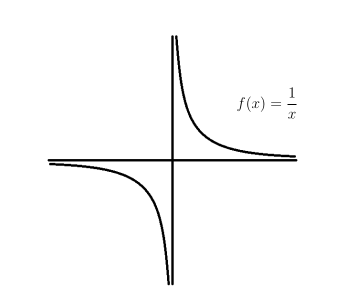
\includegraphics[scale=0.200]{LR-GrenzWert.png} \newline
Im Fall \(a \in \R\),
\[f: ]0,\infty[ \rightarrow \R\]
\[x \rightarrow x^a\]
ist f auf \(]0,\infty[\) definiert. Falls \(a > 0\) werden wir sehen, dass
\[ \lim_{x\in ]0,\infty[\rightarrow 0} f(x) = 0\]
Sei \(f: D \longrightarrow \R \) und \(x_0 \in \R \). Wir nehemn an, \(x_0\) ist Häufungspunkt von \(D \cap ]x_0, +\infty[;\)
das heisst ein rechtsseitiger Häufungspunkt. Falls der Grenzwert der eingeschränkten Funktion
\[f|_{D \cap [x_0,+\infty[}\]
für \(x \longrightarrow x_0\) existiert, wird er mit
\[ \lim_{x \rightarrow x_0^+} f(x)\]
bezeichnet und nennt sicht rechtsseitiger Grenzwert von \(f\) bei \(x_0\).\newline \newline
Wir erweitern diese Definition auf:
\[\lim_{x \rightarrow x_0^+} f(x) = +\infty \]
falls gilt:
\[ \forall \epsilon > 0 \exists \delta > 0, \ \forall x \in D \cap ]x_0,x_0 + \delta[:\ f(x) > \frac{1}{\epsilon}\]
und analog:
\[ \lim_{x \rightarrow x_0^+} f(x) = -\infty \]
falls
\[ \forall \epsilon > 0 \  \exists \delta > 0, \ \forall x \in D \cap ]x_0,x_0+\delta[: f(x) < -\frac{1}{\epsilon}\]
Linksseitige Häufungspunkt und Grenzwerte werden analog definiert. Mit diesen Definitionen gilt:
\[\lim_{x \rightarrow 0^+}\frac{1}{x} = +\infty, \quad\ \lim_{x \rightarrow 0^-}\frac{1}{x} = -\infty \] 
\Bsp[3.53] \( \lim_{x \rightarrow 0^+} \ln x = -\infty\)
Nun, \(]0,\infty[ \rightarrow R, \ x \rightarrow \ln x\) ist strikt monoton. Sei \( e^{-(n+1)} < x < e^{-n}\), dann folgt \(-(n+1) < \ln x < -n\) \newline
\Bsp[3.54] Für \( a > 0\) ist \( \lim_{x \rightarrow 0^+} x^a =0.\) Aus 5.53 folgt, dass es für jedes \(n \in \N\) ein \( \delta > 0\) gibt so dass:
\[ 0 < x < \delta \implies \ln x < -n\]
und da \( a > 0\)
\[ a \ln x < -an\]
und da \( \exp \) (streng) monoton wachsend,
\[ x^a = \exp(a \ln x) < \exp(-an)\]
Nun wird mit \(n \in \N\) beliebig gross \( \exp(-an) = (\exp(-a))^n\) beliebig klein, da \(\exp(-a) < 1\)
\section{Differenzierbare Funktionen}
\Def[4.1] Sei \( D \subseteq \R , f: D \rightarrow \R \) und \(x_0 \in D\) ein Häufungspunkt von D \newline
f ist ist \textbf{in \(x_0\) Differenzierbar}, falls der Grenzwert
\[ \lim\limits_{x \rightarrow x_0} \frac{f(x) - f(x_0)}{x - x_0}\]
existiert. Ist dies der Fall, wird der Grenzwert mit \(f'(x_0)\) bezeichnet \newline
\Bem{4.2}: Es ist oft von Vorteil in der Definiton von \(f'(x_0)\), \(x = x_0 +h\) zu setzen \[f'(x_0) = \lim_{h \rightarrow 0} \frac{f(x_0+h)-f(x_0)}{h}\]
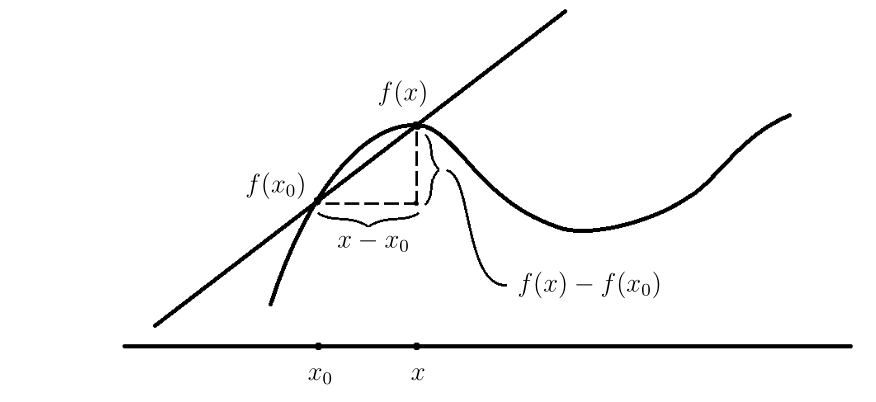
\includegraphics[scale=0.225]{differenzierbar.png} \newline
\( \frac{f(x) - f(x_0)}{x - x_0}\) ist die Steigung der Gerade durch \((x_0, f(x_0)), (x,f(x))\). Falls \(f'(x_0)\) existiert ist die Intuition, dass die Familien der Geraden durch \((x_0, f(x_0)), (x,f(x))\) für \(x \neq x_0, x \rightarrow x_0\) als "Grenzwert" die Tangente zum Graphen von f in \((x_0, f(x_0))\) annimmt.
\subsection{Die Ableitung}
\Satz[4.3](Weierstrass 1861). Sei \(f: D \rightarrow \R, x_0 \in D\) Häufungspunkt von D. Folgende Aussagen sind äquivalent:
\begin{enumerate}
    \item [1] f ist in \(x_0\) differenzierbar.
    \item [2] Es gibt \(c \in \R \) und \(r: D \rightarrow D \) mit:
    \begin{enumerate}
        \item  [2.1] \(f(x) = f(x_0) + c(x - x_0) + r(x)(x-x_0)\)
        \item  [2.2] \(r(x_0) = 0 \) und r ist stetig in \(x_0\)
    \end{enumerate} 
\end{enumerate}
Falls dies zutrifft ist \(c = f'(x_0)\) eindeutig bestimmt
Die Formulierung der Differenzierbarkeit von f mittels
\[ f(x) = f(x_0) + f'(x_0)(x - x_0) + r(x)(x - x_0)\]
und der Stetigkeit von r in \(x_0\) hat den Vorteil, dass sie keinen Limes enthält. Ausserdem ist dann
\[ y = f(x_0) + f'(x_0)(x - x_0)\]
die Gleichung der Tangente zum Graphen von f im Punkt \( (x_0, f(x_0))\).
WIr können die Charakterisierung der Differenzierbarkeit noch vereinfachen in dem wir in Satz 4.3(2.1)
\[ \phi(x) = f'(x_0) + r(x)\]
setzen. Wir erhalten: \newline
\Satz[4.4]Eine Funktion \( f: D \rightarrow \R\) ist genau dann in \(x_0\) differenzierbar, falls es eine Funktion \(\phi : D \rightarrow \R \) gibt die stetig in \(x_0\) ist und so, dass
\[f(x) = f(x_0) + \phi(x)(x - x_0) \quad \forall x \in D\]
In diesem Fall gilt \(\phi(x_0) = f'(x_0)\) \newline
\Korollar[4.5] Sei \(f : D \rightarrow \R \) und \(x_0 \in D \) ein Häufungspunkt von D. Falls \(f\) in \(x_0\) differenzierbar ist, so ist \(f\) stetig in \(x_0\) \newline
\Bsp[4.6] \begin{enumerate}
    \item  \( f = 1: \R \rightarrow \R\), dann ist \(f'(x) = 0 \quad  \forall x_0 \in \R \)
    Folgt aus \(f(x) - f(x_0) = 1 - 1 = 0\)
    \item  \( f : \R \rightarrow \R, f(x) = x\). Dann ist \(f'(x_0)=1\) \newline
    Folgt aus \(f(x) - f(x_0) = 1 \cdot (x - x_0) \)
    \item  \(f: \R \rightarrow \R, f(x) = x^2\). Dann ist \(f'(x_0) = 2x_0 \quad \forall x_0 \in \R\) \newline
    Folgt aus:
    \[ f(x) - f(x_0) = x^2 - x_0^2 = (x-x_0)(x+x_0)\]
    Also für \( x \neq x_0:\)
    \[ \frac{f(x) - f(x_0)}{x - x_0} = x + x_0\]
    woraus
    \[ \lim_{x \rightarrow x_0} \frac{f(x) - f(x_0)}{x - x_0} = \lim_{x \rightarrow x_0} (x + x_0) = 2x_0\]
    folgt.
    \item  \(f: \R \rightarrow \R, f(x) = \abs{x}\) \newline
    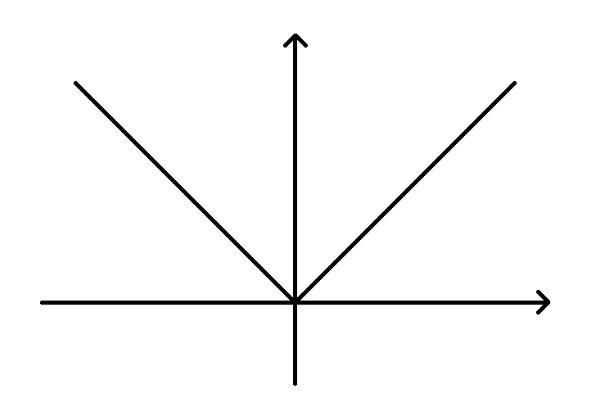
\includegraphics[scale=0.225]{ABS-function.png}
    \newline
    Ist in \(x_0 = 0\) nicht differenzierbar: \newline
    Für \( x < 0:\)
    \[ \frac{f(x) - f(0)}{x - 0} = \frac{\abs{x}}{x} = -1\]
    Für \( x > 0:\)
    \[ \frac{f(x) - f(0)}{x - 0} = \frac{\abs{x}}{x} = 1\]
    Also hat für \(x \rightarrow 0, \frac{f(x) - f(0)}{x - 0}\) keinen Grenzwert.
    Für alle \(x_0 \neq 0\) ist \(f\) in \(x_0\) differenzierbar.
    \item (Van der Waerden) Sei für \(x \in \R,\)
    \[ g(x) = \min\{\abs{x - m} : m \in \Z\}\] \newline
    \hspace*{-5mm}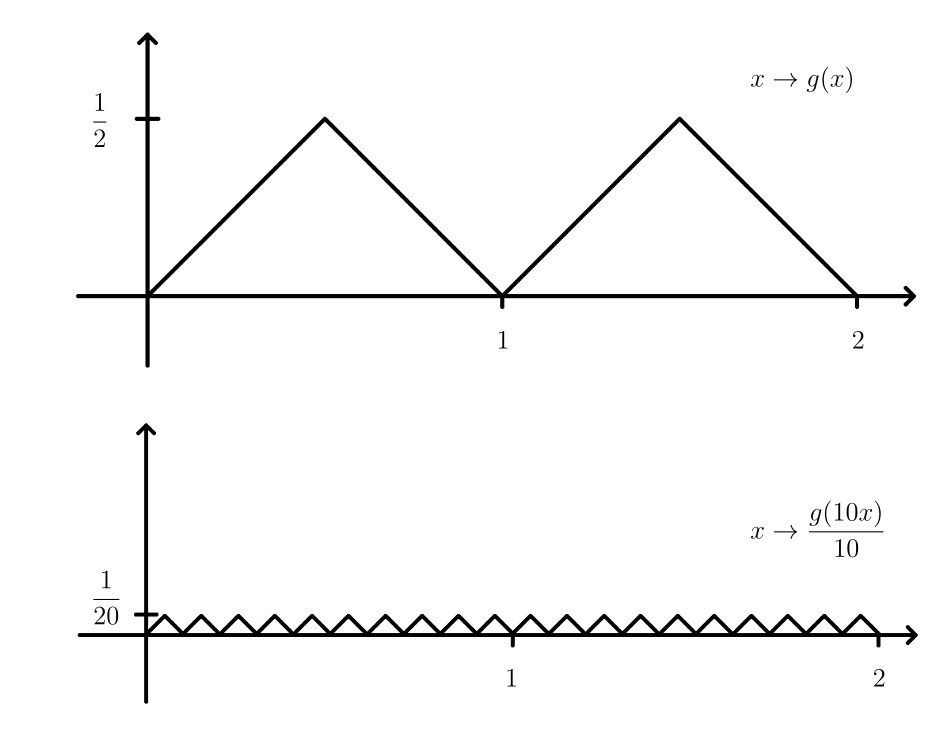
\includegraphics [scale=0.185]{VanDerWaerden.png} \newline
    Sei
    \[ f(x) = \sum_{n=0}^{\infty} \frac{g(10^nx)}{10^n}\]
    Dann ist nach Satz 3.38 diese Reihe auf ganz \( \R\) gleichmässig konvergent und \(f\) ist deswegen stetig. Mittels Dezimalentwicklung kann man zeigen, dass \(f\) in keinem Punkt von \(\R\) differenzierbar ist.
\end{enumerate}
\Def[4.7] \(f: D \rightarrow \R\) ist \textbf{in D differenzierbar}, falls für jeden Häufungspunkt \(x_0 \in D, f\) in \(x_0\) differenzierbar ist. \newline
\Bsp[4.8]
\begin{enumerate}
    \item \( \exp : \R \rightarrow \R \) ist in \( \R\) differenzierbar und \(exp' = exp\)
    Seien \(x_0 \in \R\) und \( h \neq 0:\)
    \[\frac{\exp(x_0 + h)-\exp(x_0)}{h} = \] \newline
    \[\frac{\exp(x_0)\exp(h)-\exp(x_0)}{h} = \] \newline
    \[\exp(x_0) \left[ \frac{\exp(h)-1}{h}\right]\]
    Also: \[ \exp'(x_0) = \exp(x_0) \lim_{h \rightarrow 0} \left[ \frac{\exp(h) - 1}{h}\right]\]
    Aus \( \exp(h) = 1 + h + \frac{h^2}{2!}+ \dots \) folgt für \( h \neq 0\):
    \[\frac{\exp(h) - 1}{h} = 1 + \frac{h}{2!} + \frac{h^2}{3!} + \dots\]
    und für \( h \in [-1,1], h \neq 0\):
    \[ \abs{\frac{\exp(h) - 1}{h}-1} \leq \abs{h} \left[ \frac{1}{2!} + \frac{\abs{h}}{3!} + \dots \right] \leq 2\abs{h}\]
    woraus
    \[ \lim_{h \rightarrow 0} \left( \frac{\exp(h) - 1}{h}\right) - 1 = 0\]
    folgt.
    \item \(\sin' = \cos und \cos' = -\sin\)
\end{enumerate}
\Satz[4.9] Sei \(D \subseteq \R, x_0 \in D\) ein Häufungspunkt von D und \(f,g : D \rightarrow \R \) in \(x_0\) differenzierbar. Dann gelten
\begin{enumerate}
    \item [1] \(f + g\) ist in \(x_0 \) differenzierbar und
    \[(f + g)'(x_0) = f'(x_0) + g'(x_0)\]
    \item [2] \(f \cdot g\) ist in \(x_0\) differenzierbar und
    \( (f \cdot g)'(x_0) = f'(x_0)g(x_0) + f(x_0)g'(x_0)\)
    \item [3] Falls \(g(x_0) \neq 0 \) ist \( \frac{f}{g}\) in \(x_0\) differenzierbar und
    \[ \left(\frac{f}{g}\right)'(x_0) = \frac{f'(x_0)g(x_0) - f(x_0)g'(x_0)}{g(x_0)^2}\]
\end{enumerate}
\Def{} Eine Funktion \(f: \R \rightarrow \R \) heisst \newline \textbf{gerade(resp. ungerade)}, falls \( f(-x) = f(x)\) \newline (resp. \(f(-x) = -f(x)\)) gilt für alle \( x \in \R\) \newline
\Bsp[4.10]
\begin{enumerate}
    \item \( n \geq 1: (x^n)' = nx^{n-1} \quad \forall x \in \R\)
    \item Die Tangensfunktion
    \[ \tan x = \frac{\sin x }{\cos x}, x \notin \frac{ \pi}{2} + \pi \Z\]
    ist auf ihrem Definitonsbereich differenzierbar und
    \[ \tan'(x) = \frac{1}{\cos^2(x)}\]
    \item Die Cotangensfunktion
    \[\cot x = \frac{\cos x}{\sin x}, x \notin \pi \Z\]
    ist auf ihrem Definitonsbereich differenzierbar und
    \[ cot'(x) = -\frac{1}{\sin^2(x)}\]
\end{enumerate}
\Satz[4.11] Seien \(D,E \subseteq \R\) und sei \(x_0 \in D\) ein Häufungspunkt. Sei \(f: D \rightarrow E\) eine in \(x_0\) differenzierbare Funktion so dass \(y_0 := f(x_0)\) ein Häufungspunkt von E ist, und sei \(g : E \rightarrow \R \) eine in \(y_0\) differenzierbare Funktion. Dann ist \(g \circ f : D \rightarrow \R \) in \(x_0\) differenzierbar und
\[ (g \circ f)'(x_0) = g'(f(x_0))f'(x_0)\]
\Korollar[4.12] Sei \(f : D \rightarrow E \) eine bijektive Funktion, \(x_0 \in D\) ein Häufungspunkt; wir nehem an \(f\) ist in \(x_0\) differenzierbar und \(f'(x) \neq 0\) ; zudem nehemn wir an \(f^{-1}\) ist in \(y_0 = f(x_0)\) stetig. Dann ist \(y_0\) Häufungspunkt von E, \(f^{-1}\) ist in \(y_0\) differenzierbar und
\[\left(f^{-1}\right)(y_0)= \frac{1}{f'(x_0)}\]
\newline \newline \newline \newline
\Bsp[4.13] \begin{enumerate}
    \item Die Ableitung von \(\ln : ]0, +\infty [ \rightarrow \R\) ist
    \[ \ln'(x) = \frac{1}{x}\]
    Für alle \(x \in \R \) gilt:
    \[ \ln(\exp(x)) = x\]
    S4.11 für \(f(x) = \exp x\) und \(g(y) = \ln y\)
    \[ \ln'(\exp x)\exp'(x) = 1 \quad \forall x \in \R\]
    und da \( \exp: \R \rightarrow ]0,\infty[\) bijektiv ist, folgt:
    \[ \forall y \in ]0,\infty[: \quad \ln'(y) \cdot y = 1\]
\end{enumerate}
\sep
\subsection{Erste Ableitung}
\Def[4.14] Sei \(f: D \rightarrow \R, D \subseteq \R \) und \(x_0 \in D\)
\begin{enumerate}
    \item [1] f besitzt ein lokales Maximum in \(x_0\) falls es \( \delta > 0 \) gibt mit:
    \[f(x) \leq f(x_0) \quad \forall x \in ]x_0 - \delta, x_0 + \delta [ \cap D\]
    \item [2] f besitzt ein lokales Minimum in \(x_0\) falls es \( \delta > 0 \) gibt mit:
    \[f(x) \geq f(x_0) \quad \forall x \in ]x_0 - \delta, x_0 + \delta[ \cap D\]
    \item [3] f besitzt ein lokales Extremum in \(x_0\) falls es entweder ein lokales Minimum oder Maximum von f ist.
\end{enumerate}
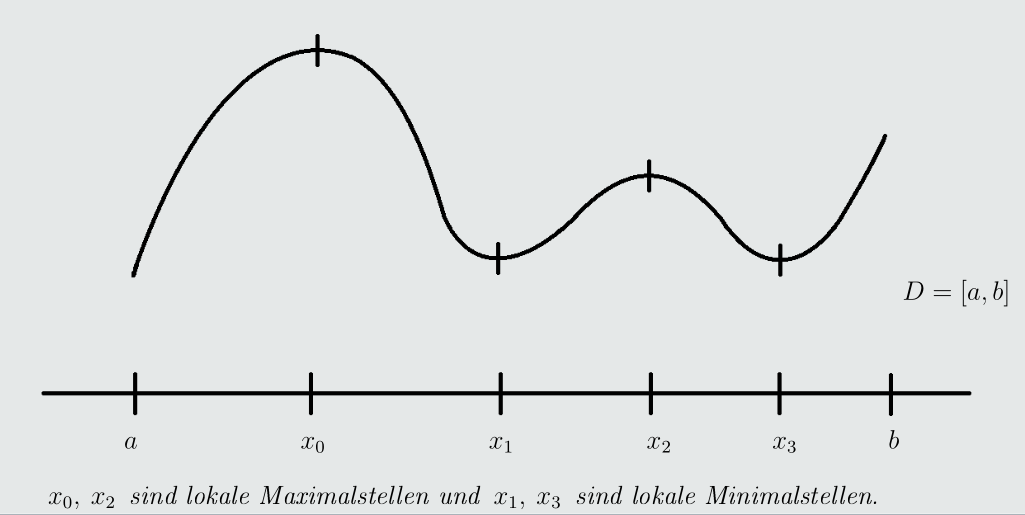
\includegraphics[scale=0.180]{MaximaMinima.png}
\Satz[4.15] Sei \(f: ]a,b[ \rightarrow \R, x_0 \in ]a,b[\). Wir nehmen an, f ist in \(x_0\) differenzierbar
\begin{enumerate}
    \item [1] Falls \(f'(x) > 0\) gibt es \( \delta > 0\) mit
    \[f(x) > f(x_0) \quad \forall x \in ]x_0,x_0 + \delta [\]
    \[f(x) < f(x_0) \quad \forall x \in ]x_0 - \delta ,x_0[\]
    \item [2] Falls \(f'(x_0) < 0 \) gibt es \( \delta > 0\) mit
    \[f(x) < f(x_0) \quad \forall x \in ]x_0,x_0 + \delta [\]
    \[f(x) > f(x_0) \quad \forall x \in ]x_0 - \delta ,x_0[\]
    \item [3] Falls f in \(x_0\) ein lokales Extremum besitzt, folgt \(f'(x_0) = 0\)
\end{enumerate}
\Satz[4.16] (Rolle 1690). Sei \(f: [a,b] \rightarrow \R \) stetig und in \(]a,b[\) differenzierbar. Erfüllt sie \(f(a) = f(b)\) so gibt es \(\mathcal{E} \in ]a,b[\) mit 
\[f'(\mathcal{E}) = 0\]
\hspace*{-3mm}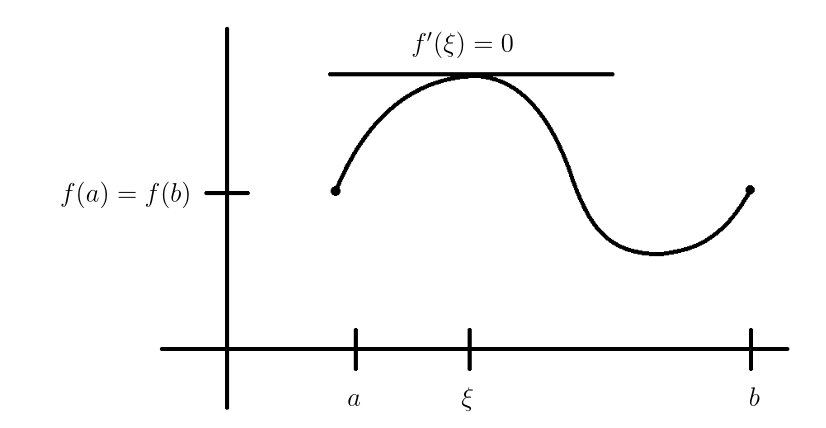
\includegraphics[scale=0.255]{SatzVonRolle.png}
\Satz[4.17] (Lagrange 1797) Sei \(f : [a.b] \rightarrow \R \) stetig mit f in \(]a,b[\) differenzierbar. Dann gibt es \( \mathcal{E} \in ]a,b[ \) mit 
\[f(b) - f(a) = f'(\mathcal{E})(b-a)\]
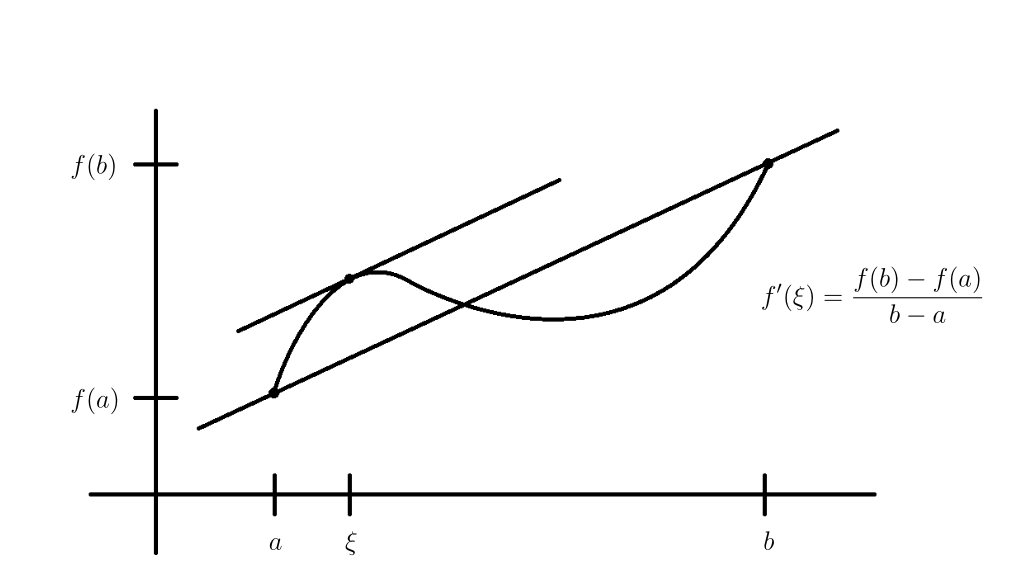
\includegraphics[scale=0.200]{Lagrange.png}
\Korollar[4.18] Seien \(f,g : [a,b] \rightarrow \R\) stetig und in \(]a,b[\) differenzierbar
\begin{enumerate}
    \item [1] Falls \[f'(\mathcal{E}) = 0 \quad \forall \mathcal{E} \in ]a,b[ \  \text{ist f konstant}\]
    \item [2] Falls \(f'(\mathcal{E}) = g'(\mathcal{E}) \quad \forall \mathcal{E} \in ]a,b[ \\ \text{gibt es c} \in \R \text{ mit} f(x) = g(x) + c \quad \forall x \in [a,b].\)
    \item [3] Falls \(f'(\mathcal{E}) \geq 0 \quad \forall \mathcal{E} \in ]a,b[ \\ \text{ist f auf } [a,b] \text{monoton wachsend}\)
    \item [4] Falls \(f'(\mathcal{E}) > 0 \quad \forall \mathcal{E} \in ]a,b[ \\ \text{ist f auf} [a,b] \text{ strikt monoton wachsend}\)
    \item [5] Falls \(f'(\mathcal{E}) \leq 0 \quad \forall \mathcal{E} \in ]a,b[ \\\text{ ist f auf } [a,b] \text{monoton fallend}\)
    \item [6] Falls \(f'(\mathcal{E}) < 0 \quad \forall \mathcal{E} \in ]a,b[ \\ \text{ist f auf } [a,b] \text{strikt monoton fallend}\)
    \item [7] Falls es \(M \geq 0 \) gibt mit
    \[\abs{f'(\mathcal{E})} \leq M \quad \forall \mathcal{E} \in ]a,b[\]
    dann folgt \( \forall x_1, x_2 \in [a,b] : \)
    \[\abs{f(x_1) - f(x_2)} \leq M \abs{x_1 - x_2}\]
\end{enumerate}
\Satz[4.22] (Cauchy). Seien \(f,g : [a,b] \rightarrow \R \) stetig und in \(]a,b[\) differenzierbar. Dann gibt es \( \mathcal{E} \in ]a.b[ \) mit 
\[ g'(\mathcal{E}) (f(b) - f(a)) = f'(\mathcal{E}) (g(b) - g(a))\]
Falls \(g'(x) \neq 0 \quad \forall x \in ]a,b[ \) folgt
\[g(a) \neq g(b)\]
und
\[\frac{f(b) - f(a)}{g(b) - g(a) } = \frac{f'(\mathcal{E})}{g'(\mathcal{E})}\]
Randnotiz: Man erhält den Satz von Lagrange mit \(g(x) = x\) \newline
\Satz[4.23] (l'Hospital 1696) Seien \(f,g : ]a,b[ \rightarrow \R \) differenzierbar mit \(g'(x) \neq 0 \quad \forall x \in ]a,b[\)\newline Falls
\[ \lim\limits_{x \rightarrow b^-}f(x) = 0, \lim\limits_{x \rightarrow b^-} g(x) = 0\]
und
\[ \lim\limits_{x \rightarrow b^-} \frac{f'(x)}{g'(x)} =: \lambda\]
existiert, folgt
\[ \lim\limits_{x \rightarrow b^-} \frac{f(x)}{g(x)} = \lim\limits_{x \rightarrow b^-} \frac{f'(x)}{g'(x)}\]
\Bem{4.24} Der Satz gilt auch 
\begin{enumerate}
    \item [$\bullet$] falls \(b = + \infty\)
    \item [$\bullet$] falls \( \lambda = + \infty\)
    \item [$\bullet$] falls \( x \rightarrow a^{+}\)
\end{enumerate}
\Bsp[4.25]
\begin{enumerate}
    \item Für \( a > 0\) folgt aus S4.13 (1), (2) und l'Hospital:
    \[ \lim_{x \rightarrow \infty} \frac{\ln x }{x^a} = \lim_{x \rightarrow \infty} \frac{\left( \frac{1}{x}\right)}{ax^{a-1}} = \lim_{x \rightarrow \infty} \frac{1}{ax^a} = 0\]
    \item \[ \lim_{x \rightarrow 0^+} x \cdot \ln x = \lim_{x \rightarrow 0^+} \frac{\ln x }{\left( \frac{1}{x}\right)} = \] 
    \[\lim_{x \rightarrow 0^+} \frac{\frac{1}{x}}{-\frac{1}{x^2}} = \lim_{x \rightarrow 0^+} (-x) = 0\]
\end{enumerate}
\Def[4.26] Sei \(I \subseteq \R \) ein Intervall und \(f: I \rightarrow \R \) eine Funktion.
\begin{enumerate}
    \item [1] f ist \textbf{konvex} (auf I) falls es für alle \newline \(x \leq y, \quad x,y \in I \) und \(\lambda \in [0,1]\) \newline
    \(f(\lambda x + (1 - \lambda)y) \leq \lambda f(x) + (1 - \lambda) f(y)\) gilt
    \item [2] f ist \textbf{streng konvex} falls für alle \newline \(x < y, \quad x,y \in I \) und \( \lambda \in ]0,1[\) \newline
    \(f(\lambda x + (1 - \lambda)y) < \lambda f(x) + (1 - \lambda)f(y)\)
\end{enumerate}
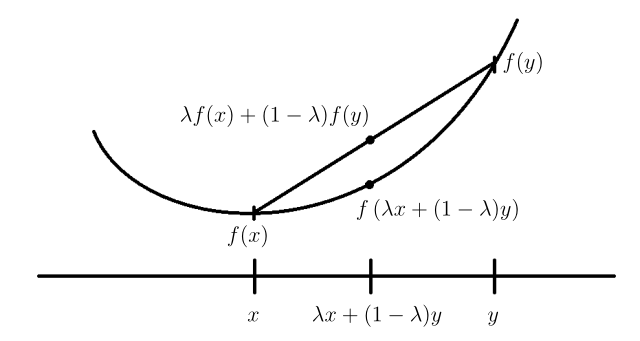
\includegraphics[scale=0.255]{Konvexität.png} \newline
\Bem{4.27} Sei \(f : I \rightarrow \R \) konvex. Ein einfacher Induktionsbeweis zeigt, dass für alle \newline \(n \geq 1, \ \{x_1, \dots x_n \} \subseteq I \) und \(\lambda_1, \dots, \lambda_n\) in \([0,1]\) mit \(\sum_{i=1}^n \lambda_i = 1\)
\[f\left(\sum_{i=1}^n \lambda_i x_i\right) \leq \sum_{i=1}^n \lambda_i f(x_i)\]
\Lemma[4.28] Sei \(f : I \rightarrow \R \) eine beliebige Funktion. Die Funktion f ist genau dann konvex, falls für alle \(x_0 < x < x_1 \) in I
\[ \frac{f(x) - f(x_0)}{x - x_0} \leq \frac{f(x_1) - f(x)}{x_1 - x}\]
gilt.\newline f ist streng konvex wenn \( < \) gilt \newline
\Satz[4.29] Sei \(f : ]a,b[ \rightarrow \R \) in \(]a,b[\) differenzierbar. Die Funktion f ist genau dann (streng) konvex, falls f' (streng) monoton wachsend ist. \newline \newline \newline
\Korollar[4.30] Sei \(f : ]a,b[ \rightarrow \R \) zweimal differenzierbar in \(]a.b[\). Die Funktion f ist (streng) konvex, falls \(f'' \leq 0\) (bzw \(f'' > 0\)) auf \(]a,b[\) \newline
\Bsp[4.31] Für alle \( n \geq 1 \) und \( x_1 \dots x_n\) in \( ]0, \infty [\) gilt
\[ \sqrt[n]{x_1 \dots x_n} \leq \frac{x_1 + \dots + x_n}{n}\]
Wir betrachten \( f(x) = - \ln x\), dann ist
\[ f'(x) = -\frac{1}{x}\]
und
\[ f''(x) = \frac{1}{x^2}, \ x \in ]0,\infty [\]
Folglich ist f konvex und aus Bem. 4.27 mit \newline \( I = ]0,\infty [\) und \( \lambda_1 = \dots = \lambda_n = \frac{1}{n}\) folgt:
\[ -\ln \left( \frac{1}{n} \sum_{i = 1}^{n} x_i\right) \leq \sum_{i=1}^{n} -\frac{1}{n} \ln x_i = -\frac{1}{n} \ln (x_1, \dots x_n)\]
\sep
\subsection{Höhere Ableitungen}
\Def[4.32] Sei \(D \subseteq \R \), so dass jedes \(x_0 \in D \) Häufungspunkt der Menge D ist. Sei \(f : D \rightarrow \R \) differenzierbar in D und f' ihre Ableitung; wir setzen \(f^{(1)} = f'\)
\begin{enumerate}
    \item [1] Für \(n \geq 2\) ist f \textbf{n-mal differenzierbar in D} falls \(f^{(n-1)}\) in D differenzierbar ist. Dann ist \( f^{(n)} := (f^{(n-1)})^{'}\) und nennt sich die n-te Ableitung von f
    \item [2] Die Funktion f ist \textbf{n-mal stetig differenzierbar in D}, falls sie n-mal differenzierbar ist und falls \( f^{(n)}\) in D stetig ist
    \item [3] Die Funktion f ist in D \textbf{glatt}, falls sie \( \forall n \geq 1\), n-mal differenzierbar ist. 
\end{enumerate}
\Bem{4.33} Es folgt aus Korollar 4.5, dass für \(n \geq 1\), eine n-mal differenzierbare Funktion \newline \((n-1)\)-mal differenzierbar ist. \newline
\Satz[4.34] Sei \( D \subseteq \R \) wie in Def. 4.32, \(n \geq 1\) und \( f,g : D \rightarrow \R \) n-mal differenzierbar in D
\begin{enumerate}
    \item [1] \(f+g\) ist n-mal differenzierbar und
    \[(f+g)^{(n)} = f^{(n)} + g^{(n)}\]
    \item [2] \(f \cdot g\) ist n-mal differenzierbar und
    \[(f \cdot g)^{(n)} = \sum_{k=0}^{n} \binom{n}{k} f^{(k)}g^{(n-k)}\]
\end{enumerate}
\Bsp[4.35]
\begin{enumerate}
    \item Die Funktionen \(\exp, \sin, \cos, \sinh, \cosh, \tanh \) sind glatt auf ganz \( \R\)
    \item Polynome sind auf ganz \( \R \) glatt.
    \item \( \ln : ]0,+\infty [ \rightarrow \R \) ist glatt;
    \[ (\ln)'(x) = \frac{1}{x} = x^{-1}, \ (\ln)''(x) = (-1)x^{-2}, \dots\]
    \[\ln^{(n)}(x) = (-1)^{n-1}(n-1)!x^{-n}, \  n \geq 1\]
\end{enumerate}
\Satz[4.36] Sei \( D \subseteq \R \) wie in Def. 4.32, \( n \geq 1 \) und \(f, g: D \rightarrow \R\) n-mal differenzierbar in D
Falls \(g(x) \neq 0 \quad \forall x \in D\), ist \(\frac{f}{g}\) in D n-mal differenzierbar
\Satz[4.37] Seien \(E,D \subseteq \R \) Teilmengen für die jeder Punkt Häufungspunkt ist. Seien \(f:D \rightarrow E\) und \(g: E \rightarrow \R \) n-mal differenzierbar. Dann ist \( g \circ f\) n-mal differenzierbar und
\[(g \circ f)^{(n)}(x) = \sum_{k=1}^n A_{n,k}(x) (g^{(k)} \circ f) (x)\]
wobei \( A_{n,k}\) ein Polynom in den Funktionen \( f', f^{(2)}, \dots , f^{(n+1-k)}\) ist
\[( g \circ f)' = (g' \circ f) \cdot f'\]
\[(g \circ f)^{(2)} = ( g^{(2)} \circ f)(f')^2 + ( g' \circ f) \cdot f^{(2)}\]
\[(g \circ f)^{(3)} = \]
\[(g^{(3)} \circ f) (f')^3 + 3(g^{(2)} \circ f)f'f^{(2)} + (g' \circ f) f^{(3)}\]

\sep
\subsection{Potenzreihen \& Taylor Approx.}
In diesem Abschnitt zeigen wir, dass grob gesagt, konvergente Potenzreihen glatte Funktionen ergeben. Die Umkehrung gilt im Allgemeinen nicht und wird durch eine schwächere Aussage (Taylor Approximation) ersetzt. \newline
\Satz[4.39] Seien  \(f_n: ]a,b[ \rightarrow \R \) eine Funktionsfolge wobei \(f_n\) einmal in \(]a,b[\) stetig differenzierbar ist \( \forall n \geq 1\). Wir nehemen an, dass sowohl die Folge \((f_n)_{n \geq 1}\) wie \((f'_n)_{n \geq 1}\) gleichmässig in \(]a,b[\) konvergieren (Def. 3.34) mit \(\lim\limits_{n \rightarrow \infty} f_n =: f \) und \(\lim\limits_{n \rightarrow \infty} f'_n =: p \). \newline
Dann ist f stetig differenzierbar und \(f' = p\) \newline
\Satz[4.40] Sei \(\sum_{k=0}^\infty c_kx^k\) eine Potenzreihen mit positivem Konvergenzradius (3.39) \(\rho > 0\). Dann ist
\[f(x) = \sum_{k=0}^\infty c_k(x - x_0)^k\]
auf \(] x_0 - \rho, x_0 + \rho [\) differenzierbar und
\[f'(x) = \sum_{k=1}^\infty kc_k(x - x_0)^{k-1}\]
für alle \( x \in ]x_0 - \rho , x_0 + \rho [\) \newline
\Korollar[4.41] Unter der Voraussetzung von Satz 4.39 ist f auf \(] x_0 - \rho, x_0 + \rho[ \) glatt und
\[f^{(j)}(x) = \sum_{k=j}^\infty c_k \frac{k!}{(k-j)!}(x - x_0)^{k-j}\]
Insbesondere ist
\[c_j = \frac{f^{(j)}(x_0)}{j!}\]
\Bsp[4.42](Cauchy 1823)\newline
Das nicht jede glatte Funktion Summe einer Potenzreihe ist, folgt aus diesem Beispiel
\[f(x)=\left\{\begin{array}{cc}
\exp \left(\frac{-1}{x^{2}}\right) & x \neq 0 \\
0 & x=0
\end{array}\right. \]
Diese Funktion ist auf ganz \( \R \) glatt und \newline \( f^{(k)}(0) = 0 \quad \forall k \geq 0\).
Da andererseits  \newline \( f(x) > 0 \quad \forall x \neq 0\), gibt es keine Potenzreihe mit positivem Konvergenzradius \( \rho \), die in \( ]-\rho, \rho [\) gegen f konvergiert. \newline
Aus Satz 4.37 folgt, dass \( \forall k \geq 0\)
\[ f^{(k)}(x) = \mathcal{P}_k \left( \frac{1}{x}\right) \exp \left( \frac{-1}{x^2}\right) \quad \forall x \neq 0\]
wobei \( \mathcal{P}_k\) ein Polynom ist.
Unter Benützung von:
\[ \lim_{x \rightarrow 0} \frac{1}{x^m} \exp \left( \frac{-1}{x^2}\right) = 0 \quad \forall m \geq 0\]
folgt mit \( f^{(k)}(0) = 0:\)
\[ f^{(k+1)}(0) = \lim_{x \rightarrow 0} \frac{f^{k}(x) - f^{(k)}(0)}{x} = \lim_{x \rightarrow 0} \frac{f^{(k)}(x)}{x} = 0\]
\Satz[4.43] Sei \(f: [a,b] \rightarrow \R\) stetig und in \(]a,b[\) \newline (n+1)-mal differenzierbar. Für jedes \(a < x \leq b \) gibt es \(\mathcal{E} \in ]a,x[ \) mit:
\[ f(x) = \sum_{k=0}^n \frac{f^{(k)}(a)}{k!}(x -a)^k + \frac{f^{(n+1)}(\mathcal{E})}{(n+1)!}(x - a)^{n+1} \]
\Korollar[4.44] (Taylor Approximatio)
Sei \(f : [c,d] \rightarrow \R \) stetig und in \(]c,d[ \) (n+1)-mal differenzierbar. Sei \( c < a < d\). Für alle \(x \in [c,d]\) gibt es \( \mathcal{E}\) zwischen x und a so dass
\[f(x) = \sum_{k=0}^n \frac{f^{(k)}(a)}{k!} (x-a)^k + \frac{f^{(n+1)}(\mathcal{E})}{(n+1)} (x-a)^{n+1}\]
Anhand dieses Korollars können wir eine präzisere Aussage über lokale Extremalstellen einer \((n+1)\)-mal differenzierbaren Funktion machen.
\Korollar[4.45] Sei \( n \geq 0,  a < x_0 < b \) und \(f: [a,b] \rightarrow \R\) in \(]a,b[\) (n+1)-mal stetig differenzierbar. Annahme: \(f'(x_0) = f^{(2)}(x_0) = \dots = f^{(n)}(x_0) = 0\)
\begin{enumerate}
    \item [1] Falls n gerade ist und \(x_0\) lokale Extremalstelle, folgt \(f^{(n+1)}(x_0) = 0\)
    \item [2] Falls n ungerade ist und \(f^{(n+1)}(x_0) > 0\) so ist \(x_0\) eine strikt lokale Minimalstelle
    \item [3] Falls n ungerade ist und \(f^{(n+1)}(x_0) < 0\) so ist \(x_0\) eine strikt lokale Maximalstelle
\end{enumerate}
\Korollar[4.46] Sei \(f : [a.b] \rightarrow \R \) stetig und in \(]a,b[\) zweimal stetig differenzierbar. Sei \(x < x_0 < b\). Annahme: \(f'(x) = 0\)
\begin{enumerate}
    \item [1] Falls \(f^{(2)}(x_0) > 0\) ist \(x_0\) strikte lokale Minimalstelle
    \item [2] Falls \(f^{(2)}(x_0) < 0\) ist \(x_0\) strikte lokale Maximalstelle
\end{enumerate}
\Bsp[4.47] Sei \(f(x) = x^4 - x^2 +1\). Wir bestimmen die lokalen Extremalstellen von f. Sei \(x_0\) eine solche; dann folgt nacht Satz 4.15(3):
\[f'(x_0) = 0, \]
das heisst
\[ 4x_0^3 - 2x_0 = 0.\]
Also gilt \(x_0 \in \left\{ -\frac{1}{\sqrt{2}}, 0, \frac{1}{\sqrt{2}}\right\}\). Nun ist \newline \( f^{(2)}(x) = 12x^2 - 2\);
\[ f^{(2)} \left( -\frac{1}{\sqrt{2}}\right) = f^{(2)}\left( \frac{1}{\sqrt{2}}\right) = 4 > 0\]
\[ f^{(2)}(0) = -2 < 0\]
Also sind \( -\frac{1}{\sqrt{2}}\) und \( \frac{1}{\sqrt{2}}\) strikte lokale Minimalstellen, und 0 strikte lokale Maximalstelle.
\sep
\section{Das Riemann Integral}
\subsection{Integrabilitätskriterien}
\Def[5.1] Eine \textbf{Partition} von I ist eine endliche Teilmenge \(P \subsetneq[a, b]\) wobei \(\{a,b\} \subseteq P\)
Eine Partition \(P'\) ist eine Verfeinerung von P falls \( P \subseteq P'\). Offensichtlich ist die Vereinigung \( P_1 \cup P_2\) zweier Partitionen wieder eine Partition, insbesondere haben zwei Partitionen immer eine gemeinsame Verfeinerung.
Sei nun \( f:[a,b] \rightarrow \R\) eine beschränkte Funktion(Def3.1(3)), das heisst es gibt \( M \geq 0\) mit \( \abs{f(x)} \leq M \ \forall x \in [a,b]\). Sei auch \( P= \{x_0, x_1, \dots, x_n\}\) eine Partition von I. Insbesondere gilt:
\[ x_0 = a < a_1 < \dots < x_n =b\]
Wir bezeichnen mit \( \delta_i := x_i - x_{i-1}, \ i \geq 1\), die Länge des Teilintervalls \([x_{i-1,x_i}] \)
Wir definieren die Untersumme
\[s(f,P) := \sum_{i=1}^n f_i \delta_i, \quad f_i = \inf_{x_{i-1} \leq x \leq x_i} f(x)\]
und die Obersumme
\[S(f,P) := \sum_{i=1}^n F_i \delta_i, \quad F_i = \sup_{x_{i-1} \leq x \leq x_i} f(x)\]
Bemerke, dass
\[ -M \leq f_i \leq F_i \leq M\]
somit sind \(s(f,P)\) und \(S(f,P)\) wohldefiniert und es gilt:
\[ -M(b-a) \leq s(f,P) \leq S(f,P) \leq M(b-a)\]
\Lemma[5.2]
\begin{enumerate}
    \item [1] Sei \(P^{'}\) eine Verfeinerung von P, dann gilt:
    \[s(f.P) \leq s(f,P^{'}) \leq S(f, P^{'}) \leq S(f,P)\]
    \item [2] Für beliebige Partitionen \(P_1, P_2\) gilt:
    \[s(f,P_1) \leq S(f, P_2)\]
\end{enumerate}
\Def[5.3] Eine beschränkte Funktion \(f: [a,b] \rightarrow \R \) ist \textbf{Riemann integrierbar} falls
\[s(f) = S(f)\]
In diesem Fall bezeichnen wir den gemeinsamen Wert von \(s(f)\) und \(S(f)\) mit
\[ \int_{a}^{b} f(x) \,dx \]
\Satz[5.4] Eine beschränkte Funtkion ist genau dann integrierbar, falls
\[ \forall \epsilon > 0 \quad \exists P \in \mathcal{P}(I) \ \text{mit} \ S(f,P) - s(f,P) < \epsilon \] 
\Satz[5.8](Du Bois-Reymond 1875)
Eine beschränkte Funktion \(f : [a,b] \rightarrow \R \) ist genau dann integrierbar, falls \( \forall \epsilon > 0 \quad \exists \delta > 0\) so dass
\[ \forall P \in P_{\delta}(I), S(f, P) - s(f, P ) < \epsilon \]
Hier bezeichnet \( P_\delta (I)\) die Menge der Partitionen P für welche \( \max_{1 \leq i \leq n} \delta_i \leq \delta\) \newline
\Korollar[5.9] Die beschränkte Funktion \(f: [a,b] \rightarrow \R \) ist genau dann integrierbar mit \(A:= \int_{a}^{b} f(x) \,dx\) falls:
\( \forall \epsilon > 0 \quad \exists \delta > 0 \) so dass \( \forall P \in p(I) \) Partition mit \( \delta(P) < \delta \) und \( \epsilon_1, \dots, \epsilon_n\) mit
\(\mathcal{E}_i \in [x_{i-1}, x_i], P= \{x_0, \dots, x_n\}\)
\[\abs{ A - \sum_{i=1}^n f(\mathcal{E_i}) ( x_i - x_{i-1}) } < \epsilon \]
\sep
\subsection{Integrierbare Funktionen}
Bis jetzt haben wir gesehen, dass konstante Funktionen sowie die Funktion \( f(x) = x\) auf jedem kompakten Intervall integrierbar sind. \newline
\Satz[5.10] Seien \(f,g : [a,b] \rightarrow \R \) beschränkt, integrierbar und \( \lambda \in \R \). Dann sind \(f+g, \lambda \cdot f, f \cdot g, \abs{f}, \max(f,g), \min(f,g) \) und \( \frac{f}{g}\) ( falls \( \abs{g(x)} \geq \beta > 0 \quad \forall x \in [a,b]\)) integrierbar \newline
\Bem{5.11} Sei \( \phi : [c,d] \rightarrow \R \) eine beschränkte Funktion. Dann ist
\[\sup_{x,y \in [c,d]} \abs{\phi(x) - \phi(y )} = \sup_{ x \in [c,d]} \phi(x) - \inf_{ x \in [c,d]} \phi(x)\]
\Korollar[5.12] Seien P,Q Polynome und \([a,b]\) ein Intervall in dem Q keine Nullstelle besitzt. Dann ist
\[ [a,b] \rightarrow \R \]
\[ x \rightarrow \frac{P(x)}{Q(x)}\]
integrierbar \newline
\Def[5.13] Eine Funktion \(f: D \rightarrow \R, \quad D \subseteq \R  \) ist in D \textbf{gleichmässig stetig}, falls
 \[ \forall \epsilon > 0 \quad \exists \delta > 0 \quad \forall x,y \in D : \]
\[ \abs{x-y} < \delta \implies \abs{f(x) - f(y)} < \epsilon \]
\Bsp[5.14] Die Funktion \( f: \R \rightarrow \R, \  x \rightarrow x^2\) ist auf \( \R \) stetig aber nicht gleichmässig stetig. \newline
\Satz[5.15] (Heine 1872). Sei \(f : [a,b] \rightarrow \R\) stetig in dem kompakten Intervall \([a,b]\). Dann ist f in \([a,b]\) gleichmässig stetig. \newline
\Satz[5.16] Sei \(f: [a,b] \rightarrow \R \) stetig. Dann ist f integrierbar \newline
\Satz[5.17] Sei \(f: [a,b] \rightarrow \R\) monoton. Dann ist f integrierbar \newline
\Bem[5.18] Seien \(a < b < c \) und \(f : [a.c] \rightarrow \R \) beschränkt mit \(f |_{[a,b]}\) und \(f |_{[b,c]}\) integrierbar. Dann ist f integrierbar und
\[ \int_{a}^{c} f(x) \,dx = \int_{a}^{c} f(x) \,dx + \int_{b}^{c} f(x) \,dx \]
\Def{} Wir erweitern unsere Definiton von Integralen
\[ \int_a^a f(x) dx = 0  \ \text{und falls} \ a < b\]
\[ \int_b^a f(x) dx := - \int_a^b f(x) dx\]
\Satz[5.19] Sei \(I \subsetneq \R \) ein kompaktes Intervall mit Endpunkten a,b sowie \(f_1, f_2 : I \rightarrow \R \)  beschränkt integrierbar und \( \lambda_1, \lambda_2 \in \R \). Dann gilt:
\[ \int_{a}^{b} ( \lambda_1 f_1(x) + \lambda_2 f_2(x)) \,dx = \]
\[\lambda_1 \int_{a}^{b} f_1(x) \,dx + \lambda_2 \int_{a}^{b} f_2(x) \,dx \]
\sep
\subsection{Ungleichungen und Mittelwertsatz}
Nebst Linearität(S5.19) hat das Riemann Integral auch eine Monotonieeigenschaft; diese wiederum führt zum Mittelwertsatz der die basis des Fundamentalsatzes der Differentialrechnung bildet.
\Satz[5.20] Seien \(f,g : [a,b] \rightarrow \R \) beschränkt integrierbar, und
\[ f(x) \leq g(x) \quad \forall x \in [a,b]\]
Dann folgt:
\[ \int_{a}^{b} f(x) \,dx \leq \int_{a}^{b} g(x) \,dx \]
\Korollar[5.21] Falls \(f: [a,b] \rightarrow \R \) beschränkt integrierbar, folgt
\[ \abs{ \int_{a}^{b} f(x) \,dx} \leq \int_{a}^{b} \abs{f(x)} \,dx \]
\Satz[5.22](Cauchy-Schwarz Ungleichung 1821)
Seien \(f,g : [a,b] \rightarrow \R \) beschränkt integrierbar. Dann gilt:
\[ \abs{\int_{a}^{b} f(x) g(x) \,dx} \leq \sqrt{\int_{a}^{b} f^2(x) \,dx} \sqrt{\int_{a}^{b} g^2(x) \,dx }\]
\Satz[5.23](Mittelwertsatz, Cauchy 1821) \newline
Sei \(f: [a,b] \rightarrow \R \) stetig. Dann gibt es \(\mathcal{E} \in [a,b]\) mit:
\[ \int_{a}^{b} f(x) \,dx = f(\mathcal{E})(b-a)\]
\Bsp[5.24] Die Stetigkeit ist eine wichtige Vouraussetzung:
Sei
\begin{equation}
f:[0,1] \longrightarrow \mathbb{R}, \quad f(x)= \begin{cases}0 & 0 \leq x<\frac{1}{2} \\ 1 & \frac{1}{2} \leq x \leq 1\end{cases}
\end{equation}
Dann ist
\[ \int_0^1 f(x) \,dx = \int_0^{\frac{1}{2}} 0 \,dx + \int_{\frac{1}{2}}^1 1 \,dx = \frac{1}{2}\]
\Satz[5.25](Cauchy 1821) Seien \(f,g : [a,b] \rightarrow \R \) wobei f stetig, g beschränkt integrierbar mit \(g(x) \geq 0 \quad \forall x \in [a,b]\). Dann gibt es \(\mathcal{E} \in [a,b] \) mit
\[ \int_{a}^{b} f(x)g(x) \,dx = f(\mathcal{E}) \int_{a}^{b} g(x) \,dx \]
\sep
\subsection{Fundamentalsatz}
Dieser Satz, auch Fundamentalsatz der Analysis genannt, besagt, dass die Ableitung die Umkehrung des Integrals ist. Dieser Satz hat vielseitige Anwendungen, unter anderem die Berechnung von Flächeninhalten und Längen von Kurven \newline
\Satz[5.26] Seien \(a < b\) und \(f: [a,b] \rightarrow \R \) stetig. Die Funktion
\[F(x) = \int_{a}^{x} f(t) \,dt \quad a \leq x \leq b\]
ist in \([a,b]\) stetig differenzierbar und
\[ F'(x) = f(x) \quad \forall x \in [a,b]\]
\Def[5.27] Sei \( a < b\) und \(f: [a,b] \rightarrow \R\) stetig. Eine Funktion \(F: [a,b] \rightarrow \R\) heisst \textbf{Stammfunktion} von f, falls F (stetig) differenzierbar in \([a,b]\) ist und \(F'=f\) in \([a,b]\) gilt \newline
\Satz[5.28] (Fundamentalsatz der Differentialrechnung) Sei \(f:[a.b] \rightarrow \R \) stetig. Dann gibt es eine Stammfunktion F von f, die bis auf eine additive Konstante eindeutig bestimmt ist und es gilt: 
\[ \int_{a}^{b} f(x) \,dx = F(b) - F(a)\]
\Bsp[5.29]
\begin{enumerate}
    \item \(f(x) = x\)
    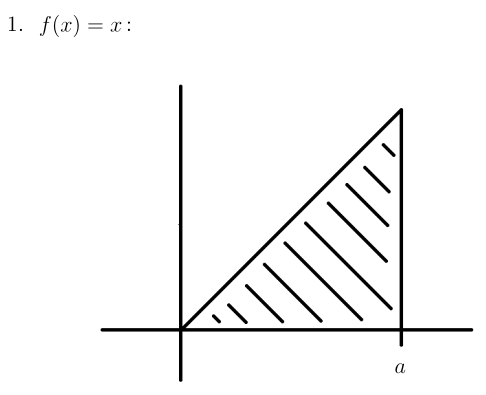
\includegraphics[scale=0.255]{Stammfunktion1.png}
    Dann ist \( \frac{x^2}{2}\) eine Stammfunktion von f und folglich:
    \[ \int_0^a x \,dx = \frac{a^2}{2} \]
    \item \(f(x) = x^2 \)
    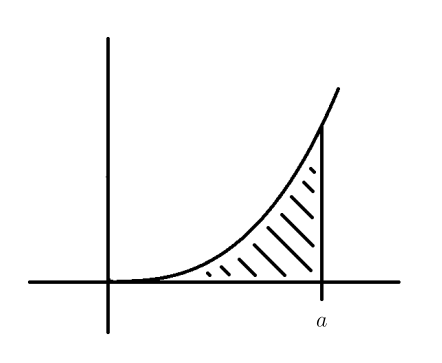
\includegraphics[scale=0.255]{Stammfunktion2.png}
    Dann ist \( \frac{x^3}{3}\) Stammfunktion von f und folglich
    \[ \int_{0}^{a} x^2 \,dx = \frac{a^3}{3}\]
\end{enumerate}
Zur Berechnung von Integralen und Stammfunktionen werden wir zwei Rechenregeln aus dem Fundamentalsatz herleiten. Es handelt sich um Partielle Integration und Substitution. \newline
\Satz[5.30](Partielle Integration) Seien \(a < b\) reele Zahlen und \(f,g : [a,b] \rightarrow \R \) stetig differenzierbar. Dann gilt
\[\int_{a}^{b} f(x)g'(x) \,dx = \] 
\[f(b)g(b) - f(a)g(a) - \int_{a}^{b} f'(x)g(x) \,dx\]
\Satz[5.31](Substitution) Sei \(a < b, \phi : [a,b] \rightarrow \R \) stetig differenzierbar, \( I \subseteq \R\) ein Intervall mit \( \phi ([a,b]) \subseteq I \) und \(f: I \rightarrow \R \) eine stetige Funktion. Dann gilt:
\[ \int_{\phi(a)}^{\phi(b)} f(x) \,dx = \int_{a}^{b} f(\phi(t))\phi'(t) \,dt\]
\Korollar[5.33] Sei \( I \subseteq \R \) ein Intervall und \(f: I \rightarrow \R\) stetig.
\begin{enumerate}
    \item [1] Seien \(a,b,c \in \R \) so dass das abgeschlossene Intervall mit Endpunkten a+c, b+c in I enthalten ist. Dann gilt:
    \[ \int_{a+c}^{b+c} f(x) \,dx = \int_{a}^{b} f(t+c) \,dt\]
    \item [2] Seien \(a,b,c \in \R \) mit \( c \neq 0\) so dass das abgeschlossene Intervall mit Endpunkten ac, bc in I enthalten ist. Dann gilt:
    \[\int_{a}^{b} f(ct) \,dt = \frac{1}{c} \int_{ac}^{bc} f(x) \,dx \]
\end{enumerate}
\sep
\subsection{Integration konvergenter Reihen}
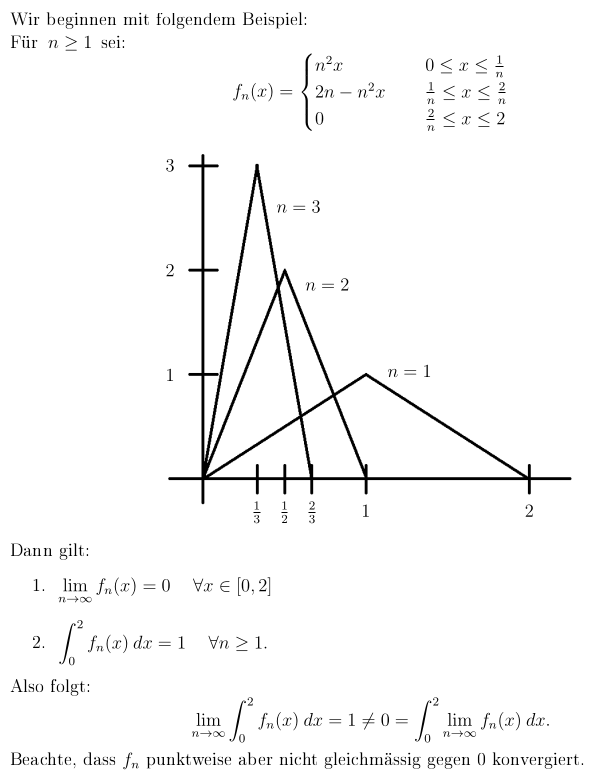
\includegraphics[scale=0.235]{Integration_konvergenterReihe.png} \newline
\Satz[5.34] Sei \(f_n : [a,b] \rightarrow \R \) eine Folge von beschränkten, integrierbaren Funktionen die gleichmässig gegen eine Funktion \(f:[a,b] \rightarrow \R \) konvergiert. Dann ist f beschränkt integrierbar und
\[ \lim\limits_{n \rightarrow \infty} \int_{a}^{b} f_n(x) \,dx = \int_{a}^{b} f(x) \,dx \]
\Korollar[5.35] Sei \(f_n : [a,b] \rightarrow \R\) eine Folge beschränkter integrierbarer Funktionen so dass
\[ \sum_{n=0}^\infty f_n\]
auf \([a.b]\) gleichmässig konvergiert. Dann gilt :
\[ \sum_{n=0}^\infty \int_{a}^{b} f_n(x) \,dx = \int_{a}^{b} \left( \sum_{n=0}^{\infty} f_n(x) \right) \,dx \]
\Korollar[5.36] Sei
\[ f(x) = \sum_{n=0}^{\infty} c_kx^k\]
eine Potenzreihe mit positivem Konvergenzradius \( \rho > 0\). Dann ist für jedes \( 0 \leq r < \rho\), f auf \([-r,r]\) integrierbar und es gilt \( \forall x \in ] -\rho, \rho[:\)
\[ \int_{0}^{x} f(t) dt = \sum_{n=0}^{\infty} \frac{c_n}{n+1} x^{n+1}\]
\sep
\subsection{Euler-McLaurin Summationsformel}
Diese Formel, ist ein sehr nützliches Instrument um Summen wie  \( 1 + \frac{1}{2} + \dots + \frac{1}{n}\)
oder \( \ln 1 + \ln 2 + \dots + \ln n = \ln n!\) abzuschätzen \newline
\Def[5.40] \( \forall k \geq 0 \) ist das k'te Bernoulli Polynom \(B_k(x) = k!P_k(x)\) Mit dieser Definition folgt: \(B_0(x) = 1, B_1(x) = x - \frac{1}{2}, B_2(x) = x^2 - x + \frac{1}{6}\)
\Def[5.41] Sei \(B_0 = 1\) für alle \( k \geq 2 \) definieren wir \(B_{k-1}\) rekursiv:
\[ \sum_{i=0}^{k-1} \binom{k}{i} B_i = 0\]
Also: \( B_0 = 1, B_0 + 2B_1 = 0, B_0 + 3B_1 + 3B_2 =0 \)
\Satz[5.42] \[ B_k(x) = \sum_{i=0}^{k} \binom{k}{i} B_ix^{k-i}\]
\Bem{5.43} Für \( k \geq 2\):

\begin{equation}
\begin{aligned}
B_{k}(1) &=\sum_{i=0}^{k}\left(\begin{array}{c}
k \\
i
\end{array}\right) B_{i}=\sum_{i=0}^{k-1}\left(\begin{array}{l}
k \\
i
\end{array}\right) B_{i}+B_{k} \\
&=B_{k} \quad(\text { nach } 5.41) \\
&=B_{k}(0) \quad(\text { nach Satz } 5.42)
\end{aligned}
\end{equation}

Zur Aussage der Summationsformel definieren wir für $k \geq 1$
$$
\widetilde{B}_{k}:[0, \infty[\longrightarrow \mathbb{R}
$$
als
$$
\widetilde{B}_{k}(x)=\left\{\begin{array}{ll}
B_{k}(x) & \text { für } \quad 0 \leq x<1 \\
B_{k}(x-n) & \text { für } n \leq x<n+1 \text { wobei } n \geq 1
\end{array}\right.
$$

\Satz[5.44] Sei \(f:[0,n] \rightarrow \R \) k-mal stetig differenzierbar, \(k \geq 1\). Dann gilt :
\begin{enumerate}
    \item [1] Für k = 1:
    \[ \sum_{i=1}^{n} f(i) = \int_{0}^{n} f(x) \,dx + \frac{1}{2} (f(n) - f(0))\]
    \[ + \int_{0}^{n} \tilde{B_1} (x) f'(x) \,dx \]
    \item [2] Für \( k \geq 2\):
    \[ \sum_{i=1}^{n}f(i) = \int_{0}^{n} f(x) \,dx + \frac{1}{2}(f(n) - f(0)) + \] 
    \[\sum_{J=2}^{k} \frac{(-1)^jB_j}{j!}(f^{(j-1)}(n) - f^{(j-1)}(0)) + \tilde{R_k}\]
    wobei
    \[ \tilde{R_k} = \frac{(-1)^{k-1}}{k!} \int_{0}^{n} \tilde{B_k}(x)f^{(k)}(x) \,dx \]
\end{enumerate}
\sep
\subsection{Stirling'sche Formel}
Die Stirling'sche Formel ist eine qualitative Aussage über das Verhalten der Fakultät
Nämlich:
\[ n! \approx \frac{\sqrt{2 \pi n} n^n}{e^n}\]
\Satz[5.47] \[n! = \frac{\sqrt{2 \pi n} n^n}{e^n} \cdot \exp(\frac{1}{12n}+ R_3(n))\]
wobei
\[ \abs{R_3(n)} \leq \frac{\sqrt{3}}{216 \cdot \frac{1}{n^2}} \quad \forall n \geq 1\]
\Lemma[5.48] \( \forall m \geq n + 1 \geq 1\):
\[ \abs{R_3(m,n)} \leq \frac{\sqrt{3}}{216}( \frac{1}{n^2} - \frac{1}{m^2})\]
\sep
\subsection{Uneigentliche Integrale}
Der Begriff des Riemann Integrals setzt voraus, dass \( [a,b]\) ein kompaktes Intervall und \(f: [a,b] \rightarrow \R \) beschränkt ist. Unter gewissen Vouraussetzungen kann man diese Einschränkung umgehen. \newline
\Def[5.49] Sei \(f:[a, \infty[ \rightarrow \R \) beschränkt und integrierbar auf \([a,b]\) für alle \( b > a\). Falls
\[ \lim\limits_{b \rightarrow \infty} \int_{a}^{b} f(x) \,dx \]
existiert, bezeichnen wir den Grenzwert mit
\[ \int_{a}^{\infty} f(x \,dx )\]
und sagen, dass f auf \([a, +\infty[ \) integrierbar ist.
\Bsp[5.50]
\begin{enumerate}
    \item \[\int_{0}^{\infty} e^{-x} d x=\lim _{b \rightarrow \infty} \int_{0}^{b} e^{-x} d x=\]
    \[\lim _{b \rightarrow \infty}\left(1-e^{-b}\right)=1\]
    \item $\int_{1}^{b} \frac{1}{x^{\alpha}} d x= \begin{cases}\ln b & \alpha=1 \\ \frac{b^{1-\alpha}-1}{1-\alpha} & \text { sonst. }\end{cases}$
\end{enumerate}
Somit: $\int_{1}^{\infty} \frac{1}{x^{\alpha}} d x=\left\{\begin{array}{cc}\text { divergiert, } & \alpha \leq 1 \\ \frac{1}{\alpha-1} & \alpha>1\end{array}\right.$
\Lemma[5.51] Sei \(f:[a, \infty [ \rightarrow \R \) beschränkt und integrierbar auf \([a,b] \quad \forall b > a\)
\begin{enumerate}
    \item [1] Falls \( \abs{f(x)} \leq g(x) \quad \forall x \geq a \) und \(g(x)\) ist auf \([a, \infty[ \) integrierbar, so ist f auf \([a, \infty[ \) integrierbar
    \item [2] Falls \( 0 \leq g(x) \leq f(x)\) und \(\int_{a}^{\infty} g(x)\) divergiert, so divergiert auch \( \int_{a}^{\infty} f(x) \,dx \)
\end{enumerate}
\Satz[5.53] (McLaurin 1742) Sei \(f : [1 , \infty[ \rightarrow [0, \infty[ \) monoton fallend. Die Reihe
\[ \sum_{n=1}^{\infty} f(n)\]
konvergiert genau dann, wenn
\[ \int_{1}^{\infty} f(x) \,dx \]
konvergiert \newline
Eine Situation die zu einem uneigentlichen Integral führt ist, falls
\[ f:]a,b[ \rightarrow \R\]
auf jedem Intervall \([a+\epsilon, b],\  \epsilon > 0 \) beschränkt und integrabel ist aber nicht notwendigerweise beschränkt auf \( ]a,b[\) \newline
\Def[5.56] In dieser Siutation ist \( f: ]a,b[ \rightarrow \R \) integrierbar falls
\[ \lim\limits_{\epsilon \rightarrow 0^{+}} \int_{a + \epsilon}^{b} f(x) \,dx \]
existiert; in diesem Fall wird der Grenzwert mit \(\int_{a}^{b} f(x) \,dx \) bezeichnet
\sep
\subsection{Die Gamma Funktion}
\Def[5.59] Für \(s > 0\) definieren wir
\[ \Gamma(s) := \int_{0}^{\infty} e^{-x}x^{s-1} \,dx\]
\Satz[5.60](Bohr-Mollerup)
\begin{enumerate}
    \item [1] Die Gamme Funktion erfüllt die Relationen
    \begin{enumerate}
        \item [(a)] \( \Gamma(1) = 1\)
        \item [(b)] \(\Gamma(s+1) = s\Gamma(s) \quad \forall s > 0 \)
        \item [(c)] \( \Gamma\) ist logarithmisch konvex, das heisst
        \[\Gamma( \lambda x + (1 - \lambda)y) \leq \Gamma(x)^{\lambda}\Gamma(y)^{1-\lambda}\]
        für alle \(x,y > 0\) und \(0 \leq \lambda \leq 1\)
    \end{enumerate}
    \item [2] Die Gamme Funktion ist die einzige Funktion \( 0, \infty[ \rightarrow ]0, \infty [\) die (a), (b) und (c) erfüllt. Darüber hinaus gilt:
    \[\Gamma(x) = \lim\limits_{n \rightarrow +\infty} \frac{n!n^x}{x(x+1) \dots (x+n)} \quad \forall x > 0\] 
\end{enumerate}
\Lemma[5.61] Sei \( \rho > 1\) und \(q > 1\) mit
\[ \frac{1}{p} + \frac{1}{q} = 1\]
Dann gilt \(\forall a,b \geq 0 \)
\[ a \cdot b \leq \frac{a^p}{p} + \frac{b^q}{q}\]
\Satz[5.62](Hölder Ungleichung). Seien \( \rho > 1\) und \( q > 1\) mit \( \frac{1}{p} + \frac{1}{q} = 1\). Für alle \(f,g : [a,b] \rightarrow \R \) stetig gilt:
\[ \int_{a}^{b} \abs{f(x)g(x)} \,dx \leq \abs{\abs{f}}_p \abs{\abs{g}}_q\]
\sep
\subsection{Das unbestimmte Integral}
\Def[Produktzerlegung]
Seien \( \alpha \pm i\beta_1. \dots , \alpha_l \pm i\beta_l\) sowie \( \gamma_1 \dots \gamma_k \) die paarweise verschiedene Wurzeln(Nullstellen) von Q,
wobei \( \alpha_j, \beta_j, \gamma_j\) reell und \(\beta_j \neq 0\). Dann lässt sich Q in ein Produkt zerlegen:
\[ Q(x) = \prod_{j=1}^l ((x- \alpha_j)^2 + \beta_j^2)^{m_j} \prod_{i=1}^k (x - \gamma_i)^{n_i}\]
\Satz[5.65] Seien P,Q Polynome mit grad(p) < grad(Q) und Q mit Produktzerlegung. Dann gibt es \( A_{ij}, B_{ij}, C_{ij}\) reelle Zahlen mit
\[ \frac{P(x)}{Q(x)} = \sum_{i=1}^l \sum_{j=1}^{m_i} \frac{(A_{ij} + B_{ij}x)}{((x - \alpha_i)^2 + \beta_i^2)^j} + \sum_{i=1}^k \sum_{j=1}^{n_i} \frac{C_{ij}}{(x - \gamma_i)^j}\]
\sep
\section{Tipps und Tricks}
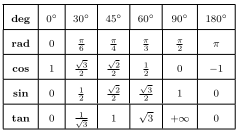
\includegraphics[scale=0.600]{RAD_values.png}
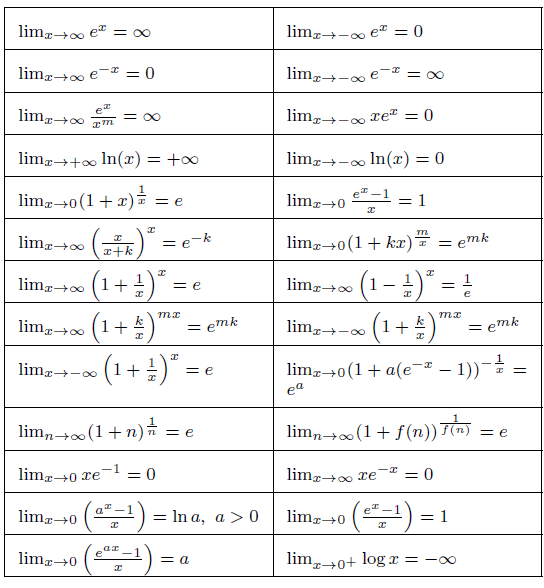
\includegraphics[scale=0.800]{RandomGrenzwerte.png}
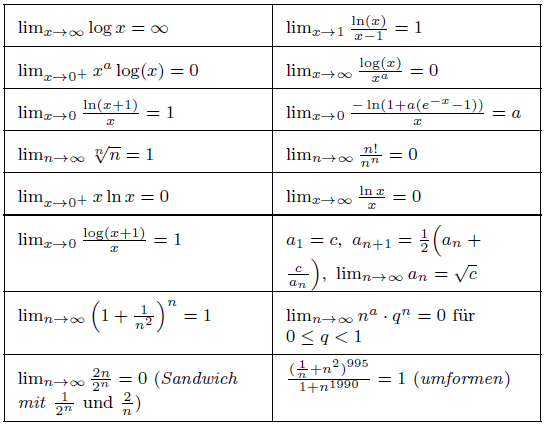
\includegraphics[scale=0.800]{randomGrenzwerte2.png}
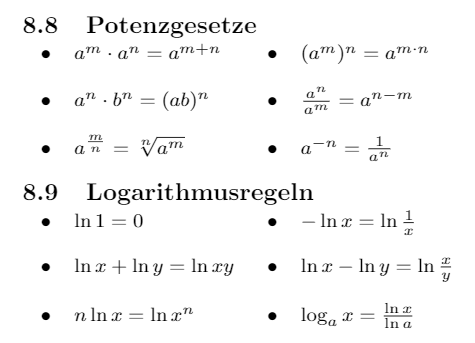
\includegraphics[scale=0.400]{logarithmus_Exponentengesetze.png}
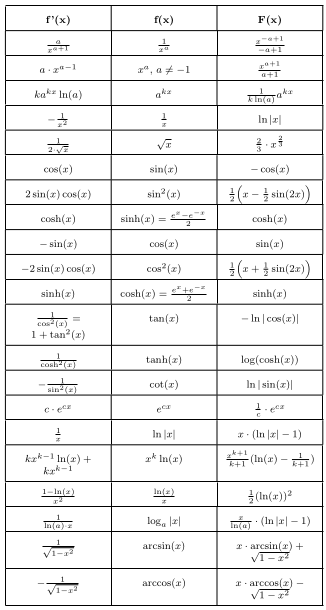
\includegraphics[scale=0.600]{randomIntegrale.png}
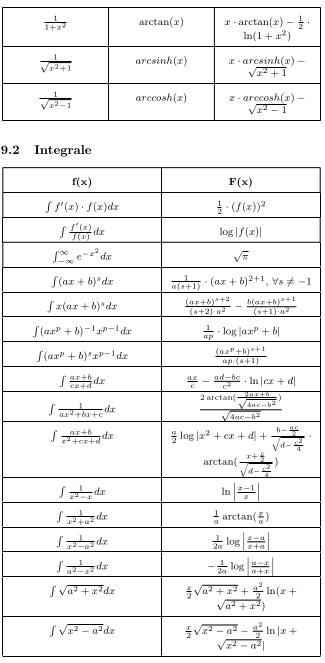
\includegraphics[scale=0.600]{randomIntegrale2.png}
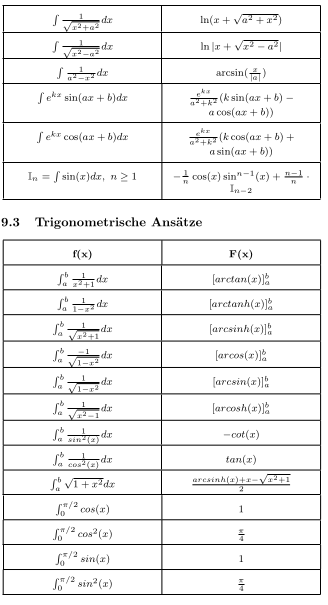
\includegraphics[scale=0.600]{randomIntegrale3.png}
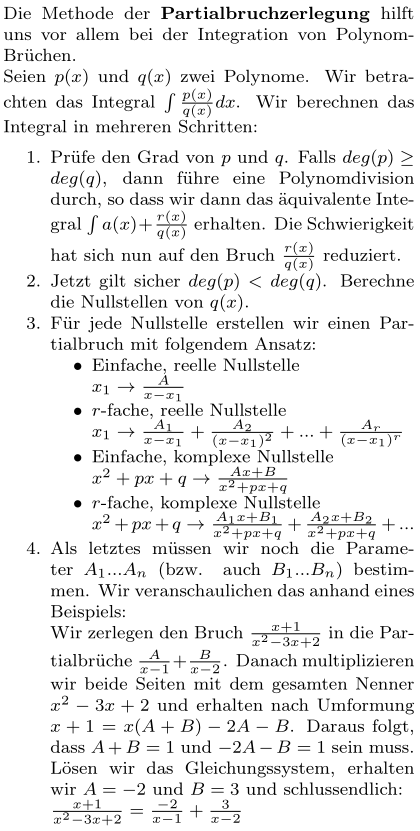
\includegraphics[scale=0.400]{Partialbruchzerlegung.png}

\end{multicols*}
\end{document}
